%%%%%%%%%%%%%%%%%%%%%%%%%%%%%%%%%%%%%%%%%%%%%%%%%%%%%%%%%%%%%%%%%%%%%%%%%%%%%%%
%DIF LATEXDIFF DIFFERENCE FILE
%DIF DEL back-up\032117\Thesis.tex   Wed Mar 29 21:28:22 2017
%DIF ADD Thesis.tex                  Wed Mar 29 21:30:00 2017
%
% THESIS DESCRIPTION:
%   A concise description of the main concepts of the thesis.
%
% RESEARCH:
%   A list of research activities which led to this thesis.
%
% EXPERIMENTS:
%   A list of the experiments performed which supported the research.
%
%%%%%%%%%%%%%%%%%%%%%%%%%%%%%%%%%%%%%%%%%%%%%%%%%%%%%%%%%%%%%%%%%%%%%%%%%%%%%%%
\documentclass[12pt,american]{report}
\usepackage{rit-thesis}
%%%%%%%%%%%%%%%%%%%%%%%%%%%%%%%%%%%%%%%%%%%%%%%%%%%%%%%%%%%%%%%%%%%%%%%%%%%%%%%
%   The following packages are all optional and depend on the specifics of what
% is contained in the thesis.  There is no harm in leaving them in.
%%%%%%%%%%%%%%%%%%%%%%%%%%%%%%%%%%%%%%%%%%%%%%%%%%%%%%%%%%%%%%%%%%%%%%%%%%%%%%%
\usepackage{subfigure}
\usepackage[refpages]{gloss}
\usepackage{babel}
\usepackage{times}
\usepackage{graphicx}
\usepackage{amssymb}
\usepackage{lscape}
\usepackage{verbatim}
\usepackage{enumerate}
\usepackage{afterpage}
\usepackage{gensymb}

\usepackage{listings}
\usepackage{fancyvrb}
\usepackage{framed}
\usepackage[listings,skins]{tcolorbox}
\usepackage[skipbelow=\topskip,skipabove=\topskip]{mdframed}
\usepackage{booktabs}
\usepackage{colortbl}

% Used for creating clicking references
\usepackage[hidelinks]{hyperref}

% Support for number sets
\usepackage{amsfonts}

\usepackage{amsmath, bm}


% Support for typesetting subcaptions
%\usepackage{subcaption}

% Support for displaying pseudo-code
\usepackage{algorithm}
%\usepackage{algorithmic}

% Support for displaying pseudo-code
%  - noend: Don't display end ...
\usepackage[noend]{algpseudocode}

% Support for pretty inline fractions
\usepackage{nicefrac}
% \end{packages}

\usepackage[listings,skins]{tcolorbox}
\usepackage{booktabs}
%\usepackage[table,xcdraw]{xcolor}
\usepackage{longtable}

\usepackage{url}


%%%%%%%%%%%%%%%%%%%%%%%%%%%%%%%%%%%%%%%%%%%%%%%%%%%%%%%%%%%%%%%%%%%%%%%%%%%%%%%
%   Mark the document as 'draft' with a date. Be sure to comment this out for
% the final version.
%\usepackage{watermark}
%\watermark{\hspace{-0.3in} \textbf{DRAFT} \hspace{2.0in} \textbf{\today}}
%%%%%%%%%%%%%%%%%%%%%%%%%%%%%%%%%%%%%%%%%%%%%%%%%%%%%%%%%%%%%%%%%%%%%%%%%%%%%%%

\makegloss
%DIF PREAMBLE EXTENSION ADDED BY LATEXDIFF
%DIF UNDERLINE PREAMBLE %DIF PREAMBLE
\RequirePackage[normalem]{ulem} %DIF PREAMBLE
\RequirePackage{color}\definecolor{RED}{rgb}{1,0,0}\definecolor{BLUE}{rgb}{0,0,1} %DIF PREAMBLE
\providecommand{\DIFaddtex}[1]{{\protect\color{blue}\uwave{#1}}} %DIF PREAMBLE
\providecommand{\DIFdeltex}[1]{{\protect\color{red}\sout{#1}}}                      %DIF PREAMBLE
%DIF SAFE PREAMBLE %DIF PREAMBLE
\providecommand{\DIFaddbegin}{} %DIF PREAMBLE
\providecommand{\DIFaddend}{} %DIF PREAMBLE
\providecommand{\DIFdelbegin}{} %DIF PREAMBLE
\providecommand{\DIFdelend}{} %DIF PREAMBLE
%DIF FLOATSAFE PREAMBLE %DIF PREAMBLE
\providecommand{\DIFaddFL}[1]{\DIFadd{#1}} %DIF PREAMBLE
\providecommand{\DIFdelFL}[1]{\DIFdel{#1}} %DIF PREAMBLE
\providecommand{\DIFaddbeginFL}{} %DIF PREAMBLE
\providecommand{\DIFaddendFL}{} %DIF PREAMBLE
\providecommand{\DIFdelbeginFL}{} %DIF PREAMBLE
\providecommand{\DIFdelendFL}{} %DIF PREAMBLE
%DIF HYPERREF PREAMBLE %DIF PREAMBLE
\providecommand{\DIFadd}[1]{\texorpdfstring{\DIFaddtex{#1}}{#1}} %DIF PREAMBLE
\providecommand{\DIFdel}[1]{\texorpdfstring{\DIFdeltex{#1}}{}} %DIF PREAMBLE
\newcommand{\DIFscaledelfig}{0.5}
%DIF HIGHLIGHTGRAPHICS PREAMBLE %DIF PREAMBLE
\RequirePackage{settobox} %DIF PREAMBLE
\RequirePackage{letltxmacro} %DIF PREAMBLE
\newsavebox{\DIFdelgraphicsbox} %DIF PREAMBLE
\newlength{\DIFdelgraphicswidth} %DIF PREAMBLE
\newlength{\DIFdelgraphicsheight} %DIF PREAMBLE
% store original definition of \includegraphics %DIF PREAMBLE
\LetLtxMacro{\DIFOincludegraphics}{\includegraphics} %DIF PREAMBLE
\newcommand{\DIFaddincludegraphics}[2][]{{\color{blue}\fbox{\DIFOincludegraphics[#1]{#2}}}} %DIF PREAMBLE
\newcommand{\DIFdelincludegraphics}[2][]{% %DIF PREAMBLE
\sbox{\DIFdelgraphicsbox}{\DIFOincludegraphics[#1]{#2}}% %DIF PREAMBLE
\settoboxwidth{\DIFdelgraphicswidth}{\DIFdelgraphicsbox} %DIF PREAMBLE
\settoboxtotalheight{\DIFdelgraphicsheight}{\DIFdelgraphicsbox} %DIF PREAMBLE
\scalebox{\DIFscaledelfig}{% %DIF PREAMBLE
\parbox[b]{\DIFdelgraphicswidth}{\usebox{\DIFdelgraphicsbox}\\[-\baselineskip] \rule{\DIFdelgraphicswidth}{0em}}\llap{\resizebox{\DIFdelgraphicswidth}{\DIFdelgraphicsheight}{% %DIF PREAMBLE
\setlength{\unitlength}{\DIFdelgraphicswidth}% %DIF PREAMBLE
\begin{picture}(1,1)% %DIF PREAMBLE
\thicklines\linethickness{2pt} %DIF PREAMBLE
{\color[rgb]{1,0,0}\put(0,0){\framebox(1,1){}}}% %DIF PREAMBLE
{\color[rgb]{1,0,0}\put(0,0){\line( 1,1){1}}}% %DIF PREAMBLE
{\color[rgb]{1,0,0}\put(0,1){\line(1,-1){1}}}% %DIF PREAMBLE
\end{picture}% %DIF PREAMBLE
}\hspace*{3pt}}} %DIF PREAMBLE
} %DIF PREAMBLE
\LetLtxMacro{\DIFOaddbegin}{\DIFaddbegin} %DIF PREAMBLE
\LetLtxMacro{\DIFOaddend}{\DIFaddend} %DIF PREAMBLE
\LetLtxMacro{\DIFOdelbegin}{\DIFdelbegin} %DIF PREAMBLE
\LetLtxMacro{\DIFOdelend}{\DIFdelend} %DIF PREAMBLE
\DeclareRobustCommand{\DIFaddbegin}{\DIFOaddbegin \let\includegraphics\DIFaddincludegraphics} %DIF PREAMBLE
\DeclareRobustCommand{\DIFaddend}{\DIFOaddend \let\includegraphics\DIFOincludegraphics} %DIF PREAMBLE
\DeclareRobustCommand{\DIFdelbegin}{\DIFOdelbegin \let\includegraphics\DIFdelincludegraphics} %DIF PREAMBLE
\DeclareRobustCommand{\DIFdelend}{\DIFOaddend \let\includegraphics\DIFOincludegraphics} %DIF PREAMBLE
\LetLtxMacro{\DIFOaddbeginFL}{\DIFaddbeginFL} %DIF PREAMBLE
\LetLtxMacro{\DIFOaddendFL}{\DIFaddendFL} %DIF PREAMBLE
\LetLtxMacro{\DIFOdelbeginFL}{\DIFdelbeginFL} %DIF PREAMBLE
\LetLtxMacro{\DIFOdelendFL}{\DIFdelendFL} %DIF PREAMBLE
\DeclareRobustCommand{\DIFaddbeginFL}{\DIFOaddbeginFL \let\includegraphics\DIFaddincludegraphics} %DIF PREAMBLE
\DeclareRobustCommand{\DIFaddendFL}{\DIFOaddendFL \let\includegraphics\DIFOincludegraphics} %DIF PREAMBLE
\DeclareRobustCommand{\DIFdelbeginFL}{\DIFOdelbeginFL \let\includegraphics\DIFdelincludegraphics} %DIF PREAMBLE
\DeclareRobustCommand{\DIFdelendFL}{\DIFOaddendFL \let\includegraphics\DIFOincludegraphics} %DIF PREAMBLE
%DIF END PREAMBLE EXTENSION ADDED BY LATEXDIFF

\begin{document}
%%%%%%%%%%%%%%%%%%%%%%%%%%%%%%%%%%%%%%%%%%%%%%%%%%%%%%%%%%%%%%%%%%%%%%%%%%%%%%%
% Title page
% The \title{} can contain line breaks as appropriate...
\title{\vspace{-0.20in}Teaching Agents with\\
  Deep Apprenticeship Learning}
% The \titleline{} must have no line breaks in it.
\titleline{Teaching Agents with Deep Apprenticeship Learning}
% There should be no reason to change the \thesistype{} or the \MSThesistrue...
\thesistype{Thesis}
\MSthesistrue
% This date is really not used (unless \grantdate{}{} is blank)
\date{May 2017}
%%%%%%%%%%%%%%%%%%%%%%%%%%%%%%%%%%%%%%%%%%%%%%%%%%%%%%%%%%%%%%%%%%%%%%%%%%%%%%%

%%%%%%%%%%%%%%%%%%%%%%%%%%%%%%%%%%%%%%%%%%%%%%%%%%%%%%%%%%%%%%%%%%%%%%%%%%%%%%%
% AUTHOR
% The \author{} should be exactly the same as your diploma
    \author{Amar Bhatt}
    \dept{Computer Engineering}
%%%%%%%%%%%%%%%%%%%%%%%%%%%%%%%%%%%%%%%%%%%%%%%%%%%%%%%%%%%%%%%%%%%%%%%%%%%%%%%

%%%%%%%%%%%%%%%%%%%%%%%%%%%%%%%%%%%%%%%%%%%%%%%%%%%%%%%%%%%%%%%%%%%%%%%%%%%%%%%
% COMMITTEE MEMBERS
% The following information is for the signature page.
% Note that the definition for principal adviser uses two fields.
% This was needed so that the adviser's name could be placed on the
% abstract page without his/her title.
%| \fivesigstrue but don't define BOTH to be true!! 
\foursigstrue

    \principaladviser{Dr. Raymond Ptucha}{Assistant Professor}
    \advdept{Computer Engineering}
    \firstreader{Dr. Ferat Sahin}{Professor}
    \firstdept{Electrical Engineering}
    \secondreader{Dr. Iris Asllani}{Assistant Professor}%
    \seconddept{Biomedical Engineering}
    \thirdreader{Louis Beato}{Lecturer}%
    \thirddept{Computer Engineering}
%%%%%%%%%%%%%%%%%%%%%%%%%%%%%%%%%%%%%%%%%%%%%%%%%%%%%%%%%%%%%%%%%%%%%%%%%%%%%%%% Use this only if \foursigstrue
%\thirdreader{Louis Beato \\ Lecturer}
%\thirdreader
% Use this only if \fivesigstrue
%\fourthreader{Reader Four \\ Reader4 Title}
%%%%%%%%%%%%%%%%%%%%%%%%%%%%%%%%%%%%%%%%%%%%%%%%%%%%%%%%%%%%%%%%%%%%%%%%%%%%%%%

%%%%%%%%%%%%%%%%%%%%%%%%%%%%%%%%%%%%%%%%%%%%%%%%%%%%%%%%%%%%%%%%%%%%%%%%%%%%%%%
% This is the expected date that the committee will sign your thesis.
\grantdate{May}{2017}
%%%%%%%%%%%%%%%%%%%%%%%%%%%%%%%%%%%%%%%%%%%%%%%%%%%%%%%%%%%%%%%%%%%%%%%%%%%%%%%

%%%%%%%%%%%%%%%%%%%%%%%%%%%%%%%%%%%%%%%%%%%%%%%%%%%%%%%%%%%%%%%%%%%%%%%%%%%%%%%
% If you want to copyright your thesis / dissertation remove the line below.
\copyrightfalse% True by default
% The year of the copyright; usually same as the date the committee will
% sign the thesis. This won't be printed if \copyrightfalse
\copyrightyear{2017}
%%%%%%%%%%%%%%%%%%%%%%%%%%%%%%%%%%%%%%%%%%%%%%%%%%%%%%%%%%%%%%%%%%%%%%%%%%%%%%%

%%%%%%%%%%%%%%%%%%%%%%%%%%%%%%%%%%%%%%%%%%%%%%%%%%%%%%%%%%%%%%%%%%%%%%%%%%%%%%%
% This causes all front matter to be set.
\beforepreface%
%%%%%%%%%%%%%%%%%%%%%%%%%%%%%%%%%%%%%%%%%%%%%%%%%%%%%%%%%%%%%%%%%%%%%%%%%%%%%%%

%%%%%%%%%%%%%%%%%%%%%%%%%%%%%%%%%%%%%%%%%%%%%%%%%%%%%%%%%%%%%%%%%%%%%%%%%%%%%%%
% The dedication - if you choose to include one.
% It should be vertically centered in the page. Since the style format doesn't
% do it for you automatically, you can use the following technique.
\prefacesection{Dedication}
\vfill
\begin{center}
To whoever...
\end{center}
\vfill
%%%%%%%%%%%%%%%%%%%%%%%%%%%%%%%%%%%%%%%%%%%%%%%%%%%%%%%%%%%%%%%%%%%%%%%%%%%%%%%

%%%%%%%%%%%%%%%%%%%%%%%%%%%%%%%%%%%%%%%%%%%%%%%%%%%%%%%%%%%%%%%%%%%%%%%%%%%%%%%
% The acknowledgements page - if you choose to include one.
% As in the dedication, it should be centered vertically in the page.
%
\prefacesection{Acknowledgments}
\vfill
\begin{center}
\indent I am grateful for ...
\end{center}
\vfill
%%%%%%%%%%%%%%%%%%%%%%%%%%%%%%%%%%%%%%%%%%%%%%%%%%%%%%%%%%%%%%%%%%%%%%%%%%%%%%%

%%%%%%%%%%%%%%%%%%%%%%%%%%%%%%%%%%%%%%%%%%%%%%%%%%%%%%%%%%%%%%%%%%%%%%%%%%%%%%%
%%  Collection of useful abbreviations.
\newcommand{\etc} {\emph{etc.\/}}
\newcommand{\etal}{\emph{et~al.\/}}
\newcommand{\eg}  {\emph{e.g.\/}}
\newcommand{\ie}  {\emph{i.e.\/}}
%%%%%%%%%%%%%%%%%%%%%%%%%%%%%%%%%%%%%%%%%%%%%%%%%%%%%%%%%%%%%%%%%%%%%%%%%%%%%%%

%%%%%%%%%%%%%%%%%%%%%%%%%%%%%%%%%%%%%%%%%%%%%%%%%%%%%%%%%%%%%%%%%%%%%%%%%%%%%%%
% Abstract
\begin{abstractpage}
As the field of robotic and humanoid systems expand, more research is being done how to best control systems to perform complex, smart tasks. Many supervised learning and classification techniques need large datasets, and only allow the system to copy what it is given. The sequential relationship within datasets used for task learning results in markov decision problems that traditional classification algorithms cannot solve. Reinforcement learning helps to solve these types of problems using a reward/punishment and exploration/exploitation methodology without the need for datasets. While this works for simple systems, complex systems are more difficult to teach using traditional reinforcement learning. Often these systems have complex, non-linear, non-intuitive cost functions which make it near impossible to model.  Inverse reinforcement learning learns complex cost functions based on input from an expert system.  This is also referred to as apprenticeship learning. Deep learning has also made a large impact in learning complex systems, and has achieved state of the art results in several applications.  Using methods from apprenticeship learning and deep learning a variety of systems can be taught complex tasks from an expert. The systems learning may not have the same degrees of freedom as the expert, but will learn how to complete the tasks based on its own functionality and limitations.
\end{abstractpage}
%%%%%%%%%%%%%%%%%%%%%%%%%%%%%%%%%%%%%%%%%%%%%%%%%%%%%%%%%%%%%%%%%%%%%%%%%%%%%%%

%%%%%%%%%%%%%%%%%%%%%%%%%%%%%%%%%%%%%%%%%%%%%%%%%%%%%%%%%%%%%%%%%%%%%%%%%%%%%%%
% Uncomment the line below if you don't want a list of tables to be printed.
% \tablespagefalse

% Uncomment the line below if you don't want a list of figures to be printed.
% \figurespagefalse

% \afterpreface generates the table of contents, list of tables (optional),
% and list of figures (optional).
\afterpreface%
%%%%%%%%%%%%%%%%%%%%%%%%%%%%%%%%%%%%%%%%%%%%%%%%%%%%%%%%%%%%%%%%%%%%%%%%%%%%%%%

\printgloss{Glossary}

%%%%%%%%%%%%%%%%%%%%%%%%%%%%%%%%%%%%%%%%%%%%%%%%%%%%%%%%%%%%%%%%%%%%%%%%%%%%%%%
% This is where the main body of the thesis starts
\body%
\chapter{Introduction}
When born, animals and humans are thrown into an unknown world forced to use their sensory inputs for survival. As they begin to understand and develop their senses they are able to  navigate  and  interact  with  their  environment.  The  process  in which  we  learn  to  do  this  is  called  reinforcement  learning.  This is  the  idea  that  learning  comes  from  a  series  of  trial  and  error where  there  exists  rewards  and  punishments  for  every  action. The brain naturally logs these events as experiences, and decides new  actions  based  on  past  experience. An  action  resulting  in  a reward  will  then  be  higher  favored  than  an  action  resulting  in a  punishment.  Using  this  concept,  autonomous  systems,  such  as robots, can learn about their environment or how to do tasks in the same way. Reinforcement learning is used in many applications aimed to reflect the way a human/animal's brain learns/reacts~\cite{atari}.  Some of these applications include the inverse pendulum, mountain car problem~\cite{sutton1996generalization}, robotic navigation, and decision based systems.  While traditional classification methods can assist in task mimicking, it does not perform well when introduced to new environments or new tasks.  Reinforcement learning does not mimic the correct move, but instead develops a policy to choose actions to obtain the highest reward.

Reinforcement learning techniques such as Q-Learning, are useful when the cost system is known, but is not the case for many complex systems. Due to the vast number of variables in tasks such as driving, walking, or medical procedures, cost functions must be learned before they are applied.  To do this, inverse reinforcement learning, or apprenticeship learning, is used. Apprenticeship learning extracts an action policy by observing an expert's transitions over time and determining the cost function from the observations~\cite{ngoinverse}. It is a Markovian decision process, in that the result of the next action is based solely on the present state and not states that happened previously. Therefore, inverse reinforcement learning sets to optimize the set of learned features in a particular state. Traditional inverse reinforcement learning uses this optimization of the linear combination of these features to determine the cost function of the given state. For static environments the traditional inverse reinforcement learning techniques are viable, however this is not the case for dynamic environments~\cite{vasquez2014inverse}. For dynamic networks, state features are constantly changing, which requires that the reward function and features be updated.   Unfortunately, this no longer gives the most optimal solution but only an approximate~\cite{vasquez2014inverse}. 

These traditional methods are not scalable to systems with large number of states.  For example, if using images as an input for reinforcement learning or apprenticeship learning, the Q-table would be very large, and often times unsustainable.  Therefore, combining these algorithms with deep learning where the rewards for state-action pairs are learned in a neural network, systems can be as complex or as large as needed~\cite{matiisen_2015}. Combining deep learning with reinforcement learning opens up a new dimension of learning, where complex correlations of environment and state features can be utilized to learn complex tasks.

\chapter{Reinforcement Learning}
Reinforcement learning is used to teach systems based on trial and error.  It uses a reward and punishment based cost function to help determine a policy on which to choose its next action.  It is based around how living creatures learn using primitive functions at a young age. This methodology creates a balance between random decisions (exploration) and choosing the best learned policy over time (exploitation). These algorithms work with agent(s), state-action pairs, and policies. An agent is what system is being operated on, such as, a car, robot, humanoid, or game solver. States represent different modes of the system, it can be any combination of environment or system specific features, such as, location of agent, location of obstacles, distance from goal, time, or speed. Actions can be anything that influences a transition from one state to another state, such as moving the agent, throwing at a target, or picking up an object.  Actions will lead to some reward/punishment that will help train the system, such as an increase/decrease in score.  Choosing an action at a specific state is called the system's policy. This is what will be learned using Reinforcement Learning.  Therefore, reinforcement learning algorithms optimize over a known cost function and output a policy.

        \subsection{Temporal Difference Learning}
        Temporal difference learning is branch of reinforcement learning that attempts to model the way an animal learns by predicting a reward in terms of a given stimulus. The heart of this algorithm comes from its prediction error signal, which constantly adjusts expected rewards based on the current given state~\cite{o2003temporal}. This algorithm estimates the value function of a state, allowing it to estimate the final reward at each state and action taken.  If it were not estimated, and instead calculated, the agent would need to wait until the final reward before updating state and action reward values. The non-estimated value function is shown in (\ref{eq:value function}) and the temporal difference estimation of the value function is shown in (\ref{eq:temporal difference value function})~\cite{Eden}. Each of these two functions return a value (\textit{V}) when given a state (\textit{s}) at time step (\textit{t}) which is represented by \textit{$s_t$}. The value \textit{$V(s_t)$} is the anticipated value or reward at specific state.  If \textit{$V(s_t)$} is very high, then that state will carry a higher importance upon evaluation. Therefore, when evaluating this type of algorithm, the next states with the largest values will be transitioned to. The learning rate, \textit{$\alpha$}, is used to determine the proportion of update.  If \textit{$\alpha$} is very large, then the update at each time step, \textit{t}, will also be large.  \textit{$R_t$} is the total reward of the system when proceeding from state \textit{$s_t$}. The immediate reward received at \textit{$s_t$} is defined by \textit{$r_t$}, therefore the reward for a state one time step out (\textit{$s_{t+1}$}) is \textit{$r_{t+1}$}. The discount rate, \textit{$\gamma$}, represents the weight (between 0 and 1) that the next state value will be multiplied with.  With a discount rate of 1, the entire value of the next state will be considered in the state value update. A discount rate of less than 1 will decrease the importance of the value of the next state in the state value update.

        \begin{equation}
            \label{eq:value function}
            V(s_{t}) = V(s_{t}) + \alpha[R_{t}-V(s_{t})]
        \end{equation}

        \begin{equation}
            \label{eq:temporal difference value function}
            V(s_{t}) = V(s_{t}) + \alpha[r_{t+1} + \gamma V(s_{t+1})-V(s_{t})]
        \end{equation}

        Estimating in this way allows for the continuous update of state values as more information is provided. As shown, the major difference between the original value function and its estimate is the consideration of the reward in the next step as well as the difference in expected reward between the current state and next state. The non-estimating function assumes that the final reward function \textit{$R_{t}$} exists as shown in (\ref{eq:discounted_reward})~\cite{matiisen_2015}.

        \begin{equation}
            \label{eq:discounted_reward}
            R_{t} = r_t + \gamma r_{t+1} + \gamma^2 r_{t+2} + ... + \gamma^{n-t}r_n 
        \end{equation}

        The \textit{r} value in (\ref{eq:temporal difference value function}) is the estimated reward for the action selected at that state in current time, whereas \textit{$R_t$} in (\ref{eq:value function}) is the final reward.  The \begin{math}\gamma\end{math} value (0 to 1) is the discount factor used for convergence, where a low \begin{math}\gamma\end{math} causes the system to over emphasize the current state, and a higher \begin{math}\gamma\end{math} will give a higher weight to future states~\cite{Eden}. Temporal difference learning requires several iterations, called episodes, to converge. An episode starts at any given state, but must end at a terminal state.  A system can have more than one terminal state (e.g. end of a game, reaching the goal state, etc.). There are two types of Temporal Difference Learning methods; Off-Policy and On-Policy.  Both methods choose a different balance between exploration and exploitation policy.  Exploration is the idea of choosing random actions to learn the entire state-space.  Exploitation is choosing only those actions that proved to be high in reward.

        
        \subsubsection{Off-Policy: Q-Learning}
        Q-learning is an off-policy method of temporal difference learning. It is the one of the most widely used algorithms in this domain. The Bellman Equation shown in (\ref{eq:bellman})~\cite{matiisen_2015} is used to update its value function denoted as \textit{Q}.

        \begin{equation}
            \label{eq:bellman}
            Q(s_{t},a_{t}) = r + \gamma*max_{a_{t+1} }(Q(s_{t+1},a_{t+1}))
        \end{equation}

        As shown, the \textit{Q-value} at state \textit{$s_t$} and \textit{$a_t$} at time step \textit{t} is based on the current value and the next best state-transitions value multiplied by the discount factor. In Q-learning \textit{Q} is represented as a table with states as its rows and actions at its columns.  Therefore, each Q-value at a particular state-action pair is the total reward at that state assuming that optimal actions are taken from that state onwards.  This requires knowledge of future states and rewards.  Therefore, this algorithm requires several episodes starting at different states to reach convergence and fill the Q-table~\cite{Watkins:1992}. This is because unlike other neural-network based applications, Q-Learning is unsupervised and must learn an environment dynamically. Typically, this causes massive overhead when scaling this algorithm to larger environments, causing the traditional Q-Learning methods to be unpopular~\cite{peng2015mobile}.  However, recent advances in this algorithm have generated new ways to define its policy making it capable to scale to larger environments~\cite{Greedy}. To iteratively update Q-values over time, the value function in (\ref{eq:Q-learning value function}) is used. 
        \begin{equation}
            \label{eq:Q-learning value function}
            Q(s_{t},a_{t}) = Q(s_{t},a_{t}) + \alpha[r_{t+1} + \gamma*max_{a_{t+1} }(Q(s_{t+1},a_{t+1}))-Q(s_{t},a_{t})]
        \end{equation}

        In this equation, \textit{$\alpha$} is the learning rate usually held between 0 and 1.  If this value is set to 1 then the Q-value is updated fully without considering the previous value, \textit{$Q(s_t,a_t)$}, which will cause the algorithm to learn very quickly. However, this may result in divergence of the algorithm.  If \textit{$\alpha$} is set to 0 then the Q-value is not updated.  Therefore, to ensure the system is learning and can converge to a solution \textit{$\alpha$} needs to be set between 0 and 1. The exact value of the learning rate needs to be determined through experimentation.

        This algorithm learns soft policies allowing it to have a high factor of exploration. Off-Policy algorithms update value functions using assumed actions which have not been tried, as shown by taking the maximum valued action at any given state.  This allows the agent to learn actions it did not actually perform~\cite{Eden}. This shows that this algorithm favors exploration more so than exploitation.  

        \subsubsection{On-Policy: Sarsa}
        Sarsa is an on-policy method of temporal difference learning~\cite{sprague2003multiple}. In this case the value function in (\ref{eq:Sarsa value function}) is updated according to a policy designed more around experience.  This ties this algorithm into considering control and exploration as one entity, whereas its Off-Policy counterpart can separate the two.

        \begin{equation}
            \label{eq:Sarsa value function}
            Q(s_{t},a_{t}) = Q(s_{t},a_{t}) + \alpha[r_{t+1} + \gamma Q(s_{t+1},a_{t+1})-Q(s_{t},a_{t})]
        \end{equation}

        Unlike the Q-Learning value function equation, Sarsa does not consider the maximum value of an action at a given state, but instead takes actions that have been taken in the past~\cite{Eden}. This shows that this algorithm favors exploitation more so than exploration. This also allows this algorithm to populate Q-values with a closer true approximate than the Q-Learning algorithm~\cite{sprague2003multiple}. Therefore, it can be said that while Q-Learning updates based on states, Sarsa updates in accordance to state-action pairs.  This allows for a better convergence policy, and leads to less unnecessary exploration by the system at hand~\cite{sutton1996generalization}.  However, because this algorithm lacks in exploration, it may converge to a local minima or non-optimal solution.

        \subsubsection{Epsilon Selection Policies}
        Both off-policy and on-policy methods of temporal difference learning rely on the selection of states and actions which is called a policy.  Policies are meant to find a balance between exploration and exploitation. Popular policies used in both Q-Learning and Sarsa are \begin{math}\epsilon\end{math}-greedy, \begin{math}\epsilon\end{math}-soft, and softmax.  In both \begin{math}\epsilon\end{math}-greedy and \begin{math}\epsilon\end{math}-soft selection policies an action is chosen with the highest estimated reward for most of the iterations. They choose a random action with a probability of \begin{math}\epsilon\end{math} for \begin{math}\epsilon\end{math}-greedy and probability 1-\begin{math}\epsilon\end{math} for \begin{math}\epsilon\end{math}-soft where \begin{math}\epsilon\end{math} is a small value between 0 to 1. \begin{math}\epsilon\end{math}-greedy is chosen to limit exploration using \begin{math}\epsilon\end{math} between 0 to 0.5. This results in 0\% to 50\% of the trials having actions chosen at random.  \begin{math}\epsilon\end{math}-soft is chosen to favor exploration using \begin{math}\epsilon\end{math} between 0 to 0.5. This results in 50\% to 100\% of the trials having actions chosen at random ~\cite{Eden}. These $\epsilon$ values can be dynamically adjusted based on number of episodes completed, number of steps within an episode, or based on how well the algorithm is converging.  Therefore, common practice is to have high exploration (random action) in the beginning of learning, and high exploitation towards the end of learning ~\cite{Greedy}.  Unlike the \begin{math}\epsilon\end{math} selections, softmax chooses random actions with respect to weights assigned to each action. These weights are adjusted over time as the system learns. This makes it so undesirable actions are less likely to be chosen over time, whereas in the \begin{math}\epsilon\end{math} selections the worst action has the same probability as the best action of being randomly chosen.  Each selection method has its own benefits, but none have proven to be better than the other~\cite{Eden}.


\section{Q-Learning and Sarsa Implementation}
Using simulated sensory data from ultrasonic sensors, moisture sensors, encoders, shock sensors, pressure sensors, and steepness sensors, a robotic system will be able to make decisions on how to navigate through its environment to reach a goal.  The robotic system will not know the source of the data or the terrain it is navigating.  Given a map of an open environment simulating an area after a natural disaster, the robot will use model-free temporal difference learning with exploration to find the best path to a goal in terms of distance, safety, and terrain navigation. Two forms of temporal difference learning will be tested; off-policy (Q-Learning) and on-policy (Sarsa). Through experimentation with several world map sizes, it is found that the off-policy algorithm, Q-Learning, is the most reliable and efficient in terms of navigating a known map with unequal states.

\subsection{Application}
In many cases robotic path planning is used in controlled environments, whether in a hospital, nursing home, hotel, etc. Reinforcement learning is also used to navigate known city maps and other open environments~\cite{peng2015mobile}. However, many of these cases fall into the category of finding the best path of a known map which can also be achieved with less invasive path planning algorithms. Consider the case of a city that underwent a natural disaster.  While the city map has stayed the same, the terrain of the city may have vastly altered. Clear roads may be flooded with water, and buildings may have been knocked down creating alternative paths. In this case, it will be pertinent for a land-based robotic system to efficiently navigate the city to reach potential resources and survivors in the safest way.  If the system took the known path as shown on a city map before the disaster, the robot may get stuck, hurt, or take too much time.  Understanding the landscape and making decisions based on the type of terrain can ensure an efficient and safe path is chosen.

\subsection{Methods}

To test the temporal difference learning algorithms, Q-Learning and Sarsa, MATLAB was used. An MxN matrix was created consisting of M*N states.  Each state had between 2-4 neighbors, depending on where on the grid it fell.  Each state also was associated to one of five terrain types; sand, forest, pavement, water, mountainous rock/debris.  These states represented an area on a map after a natural disaster.  This meaning the defined paths from a start to a goal have been severely altered. An example map is shown in Fig. \ref{fig:map-example}. Each terrain was associated to certain punishments, as decided by the simulated sensor readings on the robot.  The sensors used were, encoders (speed detection), ultrasonic sensors (visibility), shock sensor (smoothness), moisture sensor, pressure sensor (stability), and steepness sensor.  Each sensor reading was statically defined and normalized between 0 and 1, where 0 is the safest/most efficient and 1 is the most dangerous/least efficient for that particular sensor. Further testing of the system would call for the sensor readings to be introduced to natural noise.

\begin{figure}
\centering
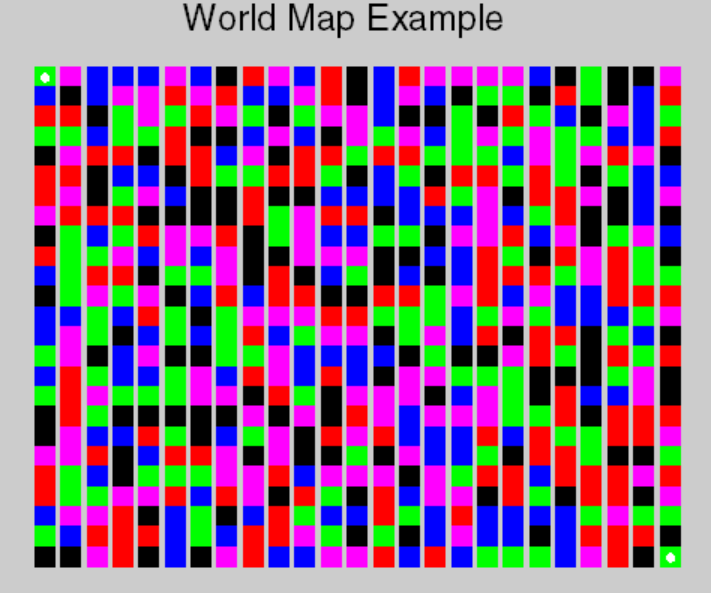
\includegraphics[scale=.5]{images/map-example.PNG}
\caption{Map Example with Terrain (Sand = Magenta, Forest = Green, Pavement = Black, Water = Blue, Misc. Debris = Red, Start/Goal = White dots)}
\label{fig:map-example}
\end{figure}

The world map matrix were at first predefined to validate the two algorithms (defined path from start to goal) and to find appropriate parameter values for the algorithms (punishment weight, discount factor, goal reward, etc).  The maps were then randomized for further testing.  The simulated robot navigating the map from the start (top left corner) to the goal (bottom right corner) had no prior knowledge of the terrain of the state it was in.  It did know the map, however.  As each algorithm was run, the value at each state was updated using a reward for the action chosen as well as a punishment which was determined by the sensor readings for each state. On a normalized average the punishments for each terrain type was as follows: sand 1, forest 2, pavement 0, water 3, mountainous rock/debris 4. This is much like the penalties incurred in James Sutton's puddle world problem, however, in this case the robot does not know about the terrain in its world, only what it reads through its sensors~\cite{sutton1996generalization}. Varying punishments made one state more favorable than another in terms of proximity to the goal, safeness, and efficiency. A rewards matrix of M*NxM*N was created, where each row symbolized a state and each column symbolized an action (next state).  Each neighbor state in the actions column were given a value of 0, non-neighbors were given a value of -\begin{math}\infty\end{math}. The goal state and any state that was a neighbor to the goal received the highest reward value.  A Q-matrix was also created the same way as the reward matrix, however, the goal was set to 0 to be updated by the temporal difference learning algorithms. Both the reward and Q-matrix represented the true map of the world without terrain information~\cite{tutorial}. Other factors needing tuning were the goal reward, the discount factor, and the punishment weight.  These were found for both algorithms through the control testing on a predefined map. Also, each algorithm was run for 10,000 episodes with an epsilon of 0.2 meaning that 20\% of the episodes would have next state actions chosen at random under the \begin{math}\epsilon\end{math}-greedy selection policy. The updated Q-matrix is used to determine the best path based on the highest rewards for each action at a given state.

\subsubsection{Q-Learning Algorithm}
To implement the Q-learning algorithm, the high-level steps outlined in Fig. \ref{fig:q-learning} were used.  As shown by the algorithm, a random state is chosen from the generated Q-matrix used to hold the values to determine the best path.  Then an action is taken in the current state based on the \begin{math}\epsilon\end{math}-greedy selection policy.  Using this action, the next state transition is determined as well as the reward for taking the action.  These values then update the Q-matrix at the current state as described by (\ref{eq:Q-learning value function}). This is then repeated with the next state, until the current state is the goal. As shown in the algorithm, the Q-matrix at each state is updated based on a learning parameter, \begin{math}\alpha\end{math} which is set to 1 in this application to assure quick learning. This matrix also depends on a discount factor denoted by \begin{math}\gamma\end{math} which is set to 0.8 to give importance to future rewards~\cite{Eden}. This was repeated for 10,000 episodes where at the start of each episode a random starting state was chosen. 
\begin{figure}
\centering
\begin{lstlisting}[frame=single]
Choose a Q(s,a)
For each episode
    Set state s
    while s is not goal
        Choose action a from s using 
            epsilon policy from Q
        Take action a, observe reward r 
            and next state s'
        Update Q-value as follows
        Q(s,a) <- Q(s,a) + $\alpha$ [r+ $\gamma$ $max_{\alpha}$(
            Q(s',a')) - Q(s,a)] (*@\newline@*)
        set s to s'
    Repeat until s is the goal state
\end{lstlisting}
\caption{Q-Learning Algorithm~\cite{Eden}}
\label{fig:q-learning}
\end{figure}



\subsubsection{Sarsa Algorithm}
To implement the Sarsa algorithm, the high-level steps outlined in Fig. \ref{fig:sarsa} were used.  As shown by the algorithm a random state is chosen from the generated Q-matrix used to hold the values to determine the best path.  Then an action is taken in the current state based on the \begin{math}\epsilon\end{math}-greedy selection policy.  Then until the state present is not the goal, the action will be taken and the next state transition is determined as well as the reward for taking the action. Another action is chosen using the \begin{math}\epsilon\end{math}-greedy selection policy for the next state. The Q-matrix at the current state is then updated as described in (\ref{eq:Sarsa value function}). As shown in the algorithm, the Q-matrix at each state is updated based on a learning parameter, \begin{math}\alpha\end{math} which is set to 1 to assure quick learning. This matrix also depends on a discount factor denoted by \begin{math}\gamma\end{math} which is set to 0.3 to give importance to future rewards~\cite{Eden}. This was repeated for 10,000 episodes where at the start of each episode a random starting state was chosen.


\begin{figure}
\centering
\begin{lstlisting}[frame=single]
Choose a Q(s,a)
For each episode
    Set state s
    Choose action a from s using epsilon 
        policy from Q
    while s is not goal
        Take action a, observe reward r 
            and next state s'
        Choose action a' from s' using 
            epsilon policy from Q
        Update Q-value as follows
        Q(s,a) <- Q(s,a) + $\alpha$ [r+$\gamma$ Q(s',a') 
            - Q(s,a)]
        set s to s'
        set a to a'
    Repeat until s is the goal state
\end{lstlisting}
\caption{Sarsa Algorithm~\cite{Eden}}
\label{fig:sarsa}
\end{figure}

\subsection{Results}

To validate the effectiveness of the two algorithms, each was run with a 5x5, 10x10, 15x15, and 25x25 size world with randomly generated terrains.  Each was run in 10 different terrain maps at each world size.  The results from this can be found in Table \ref{tab:results}.  As shown, it is apparent that the Q-Learning algorithm performs best in terms of cost.  It chooses the shortest and safest path. Also, as the world size gets bigger, the Q-Learning algorithm takes advantage of the increase in space and terrain to lower its cost per move. Sarsa also does this, but only slightly.  The Sarsa algorithm is the fastest, while it may not be the most efficient.  It is shown to finish well before the Q-Learning algorithm on larger maps.  However, the Q-Learning algorithm has a higher rate of convergence, where the Sarsa algorithm is prone to diverge at larger map sizes.  In the 25x25 world size, the Sarsa algorithm failed to converge, increasing the discount factor for the algorithm at this world size to 0.8 allowed for convergence. Examples of paths found by the Q-Learning algorithm and Sarsa algorithm at a world size of 25x25 are shown in Fig. \ref{fig:q-learning example} and Fig. \ref{fig:sarsa_example}, respectively.

In consideration of natural disaster relief and rebuilding, the Q-Learning algorithm is the best.  It takes the longest to converge, but will find the most efficient path, that is time conscience and safe for itself.  Sarsa, tends to favor the goal over safety in these situations because of its exploitation over exploration strategy. 


\begin{figure}
\centering
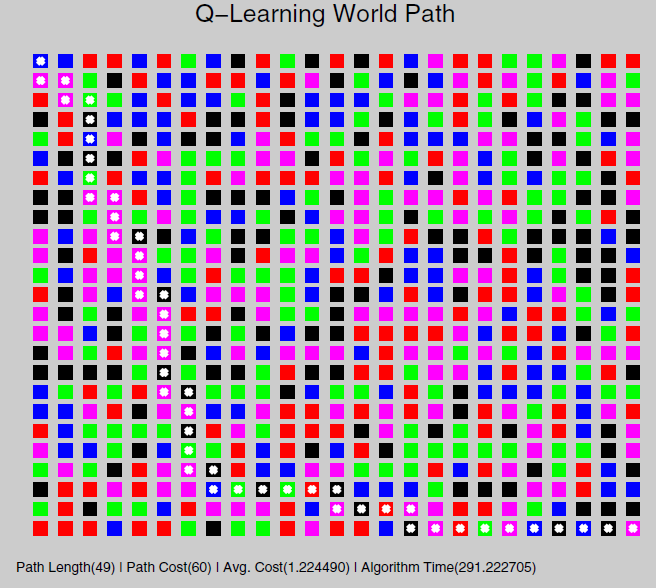
\includegraphics[scale=.5]{images/q-learning-example.PNG}
\caption{Q-Learning Algorithm Path Example with Punishment}
\label{fig:q-learning example}
\end{figure}

\begin{figure}
\centering
%\captionsetup{justification=centering}
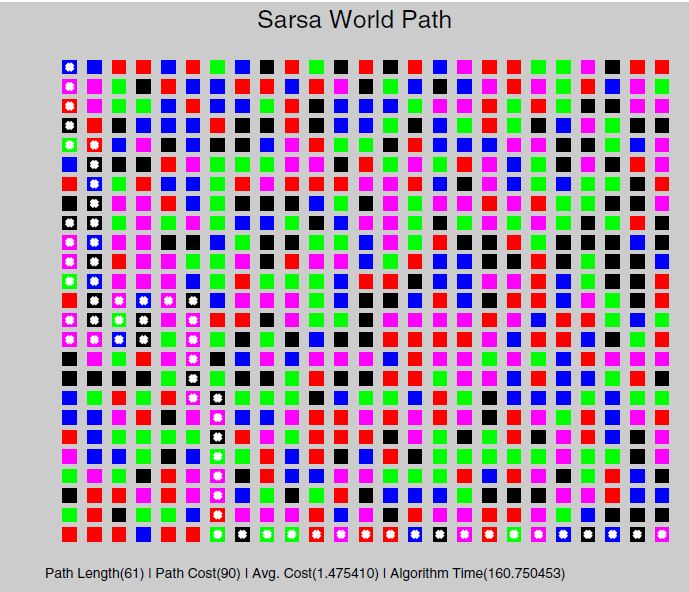
\includegraphics[scale=.5]{images/sarsa-example.PNG}
\caption{Sarsa Algorithm Path Example with Punishment}
\label{fig:sarsa_example}
\end{figure}

\begin{table}[]
\centering
%\captionsetup{justification=centering}
\caption{Q-Learning and Sarsa results across several world map sizes}
\label{tab:results}
\begin{tabular}{@{}llll@{}}
\toprule
\rowcolor[HTML]{FFFFFF} 
{\color[HTML]{333333} } & {\color[HTML]{333333} } & {\color[HTML]{333333} \textbf{Q-Learning}} & {\color[HTML]{333333} \textbf{Sarsa}} \\ \midrule
\rowcolor[HTML]{FFFFFF} 
\multicolumn{1}{|l|}{\cellcolor[HTML]{FFFFFF}{\color[HTML]{333333} }} & {\color[HTML]{333333} Avg. Path} & {\color[HTML]{333333} 9} & \multicolumn{1}{l|}{\cellcolor[HTML]{FFFFFF}{\color[HTML]{333333} 9}} \\
\rowcolor[HTML]{FFFFFF} 
\multicolumn{1}{|l|}{\cellcolor[HTML]{FFFFFF}{\color[HTML]{333333} }} & {\color[HTML]{333333} Avg. Cost} & {\color[HTML]{333333} 12.3} & \multicolumn{1}{l|}{\cellcolor[HTML]{FFFFFF}{\color[HTML]{333333} 18}} \\
\rowcolor[HTML]{FFFFFF} 
\multicolumn{1}{|l|}{\cellcolor[HTML]{FFFFFF}{\color[HTML]{333333} 5x5}} & {\color[HTML]{333333} Avg. Unit Cost} & {\color[HTML]{333333} 1.3667} & \multicolumn{1}{l|}{\cellcolor[HTML]{FFFFFF}{\color[HTML]{333333} 2.000}} \\
\rowcolor[HTML]{FFFFFF} 
\multicolumn{1}{|l|}{\cellcolor[HTML]{FFFFFF}{\color[HTML]{333333} }} & {\color[HTML]{333333} Avg. Time (s)} & {\color[HTML]{333333} 2.396} & \multicolumn{1}{l|}{\cellcolor[HTML]{FFFFFF}{\color[HTML]{333333} 2.2731}} \\
\rowcolor[HTML]{FFFFFF} 
\multicolumn{1}{|l|}{\cellcolor[HTML]{FFFFFF}{\color[HTML]{333333} }} & {\color[HTML]{333333} \% Converge} & {\color[HTML]{333333} 100} & \multicolumn{1}{l|}{\cellcolor[HTML]{FFFFFF}{\color[HTML]{333333} 100}} \\ \midrule
\rowcolor[HTML]{FFFFFF} 
\multicolumn{1}{|l|}{\cellcolor[HTML]{FFFFFF}{\color[HTML]{333333} }} & {\color[HTML]{333333} Avg. Path} & {\color[HTML]{333333} 19} & \multicolumn{1}{l|}{\cellcolor[HTML]{FFFFFF}{\color[HTML]{333333} 23.667}} \\
\rowcolor[HTML]{FFFFFF} 
\multicolumn{1}{|l|}{\cellcolor[HTML]{FFFFFF}{\color[HTML]{333333} }} & {\color[HTML]{333333} Avg. Cost} & {\color[HTML]{333333} 23.4} & \multicolumn{1}{l|}{\cellcolor[HTML]{FFFFFF}{\color[HTML]{333333} 38.8}} \\
\rowcolor[HTML]{FFFFFF} 
\multicolumn{1}{|l|}{\cellcolor[HTML]{FFFFFF}{\color[HTML]{333333} 10x10}} & {\color[HTML]{333333} Avg. Unit Cost} & {\color[HTML]{333333} 1.2316} & \multicolumn{1}{l|}{\cellcolor[HTML]{FFFFFF}{\color[HTML]{333333} 1.6260}} \\
\rowcolor[HTML]{FFFFFF} 
\multicolumn{1}{|l|}{\cellcolor[HTML]{FFFFFF}{\color[HTML]{333333} }} & {\color[HTML]{333333} Avg. Time (s)} & {\color[HTML]{333333} 12.7255} & \multicolumn{1}{l|}{\cellcolor[HTML]{FFFFFF}{\color[HTML]{333333} 12.2337}} \\
\rowcolor[HTML]{FFFFFF} 
\multicolumn{1}{|l|}{\cellcolor[HTML]{FFFFFF}{\color[HTML]{333333} }} & {\color[HTML]{333333} \% Converge} & {\color[HTML]{333333} 100} & \multicolumn{1}{l|}{\cellcolor[HTML]{FFFFFF}{\color[HTML]{333333} 60}} \\ \midrule
\rowcolor[HTML]{FFFFFF} 
\multicolumn{1}{|l|}{\cellcolor[HTML]{FFFFFF}{\color[HTML]{333333} }} & {\color[HTML]{333333} Avg. Path} & {\color[HTML]{333333} 29} & \multicolumn{1}{l|}{\cellcolor[HTML]{FFFFFF}{\color[HTML]{333333} 60.75}} \\
\rowcolor[HTML]{FFFFFF} 
\multicolumn{1}{|l|}{\cellcolor[HTML]{FFFFFF}{\color[HTML]{333333} }} & {\color[HTML]{333333} Avg. Cost} & {\color[HTML]{333333} 32.2} & \multicolumn{1}{l|}{\cellcolor[HTML]{FFFFFF}{\color[HTML]{333333} 80.0}} \\
\rowcolor[HTML]{FFFFFF} 
\multicolumn{1}{|l|}{\cellcolor[HTML]{FFFFFF}{\color[HTML]{333333} 15x15}} & {\color[HTML]{333333} Avg. Unit Cost} & {\color[HTML]{333333} 1.1103} & \multicolumn{1}{l|}{\cellcolor[HTML]{FFFFFF}{\color[HTML]{333333} 1.3110}} \\
\rowcolor[HTML]{FFFFFF} 
\multicolumn{1}{|l|}{\cellcolor[HTML]{FFFFFF}{\color[HTML]{333333} }} & {\color[HTML]{333333} Avg. Time (s)} & {\color[HTML]{333333} 37.8544} & \multicolumn{1}{l|}{\cellcolor[HTML]{FFFFFF}{\color[HTML]{333333} 33.4482}} \\
\rowcolor[HTML]{FFFFFF} 
\multicolumn{1}{|l|}{\cellcolor[HTML]{FFFFFF}{\color[HTML]{333333} }} & {\color[HTML]{333333} \% Converge} & {\color[HTML]{333333} 100} & \multicolumn{1}{l|}{\cellcolor[HTML]{FFFFFF}{\color[HTML]{333333} 40}} \\ \midrule
\rowcolor[HTML]{FFFFFF} 
\multicolumn{1}{|l|}{\cellcolor[HTML]{FFFFFF}{\color[HTML]{333333} }} & {\color[HTML]{333333} Avg. Path} & {\color[HTML]{333333} 49} & \multicolumn{1}{l|}{\cellcolor[HTML]{FFFFFF}{\color[HTML]{333333} 63.2*}} \\
\rowcolor[HTML]{FFFFFF} 
\multicolumn{1}{|l|}{\cellcolor[HTML]{FFFFFF}{\color[HTML]{333333} }} & {\color[HTML]{333333} Avg. Cost} & {\color[HTML]{333333} 51.3} & \multicolumn{1}{l|}{\cellcolor[HTML]{FFFFFF}{\color[HTML]{333333} 101*}} \\
\rowcolor[HTML]{FFFFFF} 
\multicolumn{1}{|l|}{\cellcolor[HTML]{FFFFFF}{\color[HTML]{333333} 25x25}} & {\color[HTML]{333333} Avg. Unit Cost} & {\color[HTML]{333333} 1.0469} & \multicolumn{1}{l|}{\cellcolor[HTML]{FFFFFF}{\color[HTML]{333333} 1.6005*}} \\
\rowcolor[HTML]{FFFFFF} 
\multicolumn{1}{|l|}{\cellcolor[HTML]{FFFFFF}{\color[HTML]{333333} }} & {\color[HTML]{333333} Avg. Time (s)} & {\color[HTML]{333333} 337.8118} & \multicolumn{1}{l|}{\cellcolor[HTML]{FFFFFF}{\color[HTML]{333333} 186.467*}} \\
\rowcolor[HTML]{FFFFFF} 
\multicolumn{1}{|l|}{\cellcolor[HTML]{FFFFFF}{\color[HTML]{333333} }} & {\color[HTML]{333333} \% Converge} & {\color[HTML]{333333} 100} & \multicolumn{1}{l|}{\cellcolor[HTML]{FFFFFF}{\color[HTML]{333333} 50*}} \\
\multicolumn{1}{|l|}{} & \multicolumn{3}{l|}{*with a discount factor of 0.8} \\ \bottomrule
\end{tabular}
\end{table}


\subsection{Conclusion}

Reinforcement learning is a series of methods and algorithms used to pseudo map out the way a living being makes decisions. Just like a living being, a decision cannot be proven right or wrong until it has been made~\cite{tutorial}. This methodology gives way for a system to learn its environment and discover patterns not easily recognizable. Used in the case of natural disaster response or ruins exploration, reinforcement learning, specifically temporal difference learning, can be used to explore the area, as well as build an efficient navigation map. In terms of the experiments done in this paper Q-Learning does much better than Sarsa in creating an efficient and safe path from a start to a goal.  Using multiple synchronized systems across a map, where each system would represent an episode, could reduce the time limitation found in Q-learning.  In this type of problem, Q-Learning does the best because of the importance it places on exploration.  On known, non-variable maps, Sarsa will do better because it can exploit rewards in future states early.




\chapter{Apprenticeship Learning (Inverse Reinforcement Learning)}
	Apprenticeship Learning, or inverse reinforcement learning, is the process of learning a cost/reward function to move from state to state. In these cases, the system observes and attempts to learn from another system that performs some task. Unlike reinforcement learning, the cost-function does not need to be known. Therefore, this type of system takes in an expert's policy (through demonstration) and learns a cost function based on its own state features and features perceived from the expert~\cite{jangir_2016}.		

		In \cite{hamahata2008effective} an imitation learning (inverse reinforcement learning) algorithm is used in two ways, one with supervised learning and one with reward shaping. In supervised learning, the imitator observes a demonstrator's motion and attempts to model it. One issue with this is that this is a black box learning technique.  The imitator can observe the final state of the demonstrator, but it has no knowledge of hidden states and actions used to create the motion. This can be mitigated if the imitator knows the inverse model of the demonstrator system. Hamahata et al. \cite{hamahata2008effective}, assumes that the imitator obtains the estimated actions over a discrete time from the demonstrator.  This then allows the imitator to find the optimal control to imitate the demonstrator using least squares or ridge regression. In reward shaping a more implicit approach to imitation learning is used. This method attempts to create a reward function from the observations of the demonstrator.  In many cases, changing a rewards function also changes the optimal policy of the system.  However, the rewards function found is designed to be included as an aggregate term to the underlying rewards function. The additional rewards function is defined as (~\ref{eq:additional_rewards}).
		\begin{equation}
            \label{eq:additional_rewards}
            \resizebox{0.44\textwidth}{!}{$r\textsuperscript{sub}\textsubscript{t+1}= \gamma\phi(x_{t+1})-\phi(x_{t})$}~\cite{hamahata2008effective}
        \end{equation}
		The value of this is added to the value of the underlying rewards function. In the additional rewards function, the \textit{$\phi$} term is defined when it is equal to the optimal value function. Using this shaping method the imitator has a faster learning rate~\cite{hamahata2008effective}.

		One challenge of inverse reinforcement learning is limited demonstrations and not performing the exact task as the demonstrator. In these cases, traditional imitation learning is not a feasible option. In \cite{atkeson1997robot} a method is proposed to learn an optimal policy rather than just a reward. This means that the system learns at the task level rather than just matching patterns which is useful for cases where the exact motion of the demonstrator is not learned. This paper explores the inverse pendulum problem, and attempts to solve it using reinforcement learning. This approach proved to be limited by intricately complex movements, however it did demonstrate a sense of learned movement from demonstration~\cite{atkeson1997robot}.

\section{Related Work}
\DIFaddbegin \subsection{\DIFadd{Bayesian Inverse Reinforcement Learning}}

\subsection{\DIFadd{Gaussian Process Inverse Reinforcement Learning}}

\DIFaddend \subsection{Maximum Entropy Inverse Reinforcement Learning}
\label{sec:maxentirl}
In many imitation learning problems modeling sequential decision-making behavior is often very difficult due to the lack of foresight in these systems. Ziebart et al.~\cite{ziebart2008maximum} developed an inverse reinforcement technique based on the principle of maximum entropy theory to counter this.  They tackled modeling real-world navigation and driving behaviors by sampling noisy and imperfect data from driving "experts".  Their approach was able to model route preferences of drivers as well as infer destinations and routes based on partial trajectories using GPS data of taxi-cab driving.  The environment they tested in was a known-fixed structure of the world (such as a road network) with known actions characterized by various road features such as speed limit and number of lanes.

The idea of inverse reinforcement learning revolves on an agent optimizing a function that linearly maps features of each state (\textit{$s_j$} to a reward value. Therefore, the reward value of an "expert" data sample, or trajectory, is a sum of state rewards which can be simplified to the reward weights, (\textit{$\theta$}), applied to the feature counts in a trajectory/path ($\zeta$) (\ref{eq:feature_counts}) as shown in (\ref{eq:feature_count_reward}).

\begin{equation}
            \label{eq:feature_counts}
            \resizebox{0.20\textwidth}{!}{$f\textsubscript{$\zeta$}= \sum_{s_j\in\zeta}^{}f\textsubscript{$s_j$}$}~\cite{ziebart2008maximum}%
        \end{equation}

\begin{equation}
            \label{eq:feature_count_reward}
            \resizebox{0.44\textwidth}{!}{$reward(f\textsubscript{$\zeta$})= \theta \cdot f\textsubscript{$\zeta$} = \sum_{s_j\in\zeta}^{}\theta \cdot f\textsubscript{$s_j$}$}~\cite{ziebart2008maximum}
        \end{equation}

A major problem of using "expert" trajectories is that an inverse reinforcement algorithm may find a preference for one path over others.  This poses a problem that an agent will only learn a path and not how features of a state can help in path decision making.  Using maximum entropy this problem is solved by choosing a distribution that does not exhibit preference beyond feature expectations.  Using this probabalistic model for deterministic (no randomness) path distributions, trajectories with the same final reward will be treated equally, where a preference will only be given for trajectories with higher reward.  Trajectories with a higher reward will have an exponentially higher probability. This is shown in (\ref{eq:maximum_entropy}), where \textit{Z($\theta$)} is the partition function which will always converge given trajectories that reach a reward-giving goal in a finite number of steps.

\begin{equation}
            \label{eq:maximum_entropy}
            \resizebox{0.44\textwidth}{!}{$reward(P(\zeta\textsubscript{i})|\theta)= \frac{1}{Z(\theta)} e^{\theta \cdot f_{\zeta_i}}=  \frac{1}{Z(\theta)} e^{\sum_{s_j\in\zeta_i}^{}\theta \cdot f\textsubscript{$s_j$}}$}~\cite{ziebart2008maximum}%
        \end{equation}

For non-deterministic (randomness) path distributions, (\ref{eq:maximum_entropy}) must be altered to take randomness in path distributions into account. Most MDPs (Marko Decision Process) that relate to real-world environments or dynamics will have non-deterministic transitions between states, meaning that an action that is supposed to transition to one state may not do so with some probability $\epsilon$.  Therefore, this distribution over paths produces a stochastic policy where the probability of an action is weighted by the expected rewards of all paths that begin with that action as shown in (\ref{eq:stochastic_policy}).

\begin{equation}
            \label{eq:stochastic_policy}
            \resizebox{0.44\textwidth}{!}{$reward(P(action | \theta, T) \propto \sum_{\zeta:action\in\zeta_{t=0}}^{}P(\zeta | \theta, T)$}~\cite{ziebart2008maximum}%
        \end{equation}

Therefore, to find the optimal weights the likelihood of the observed data is maximized under the maximum entropy distribution (\ref{eq:maxent_weight_update}). Since this function will be convex for deterministic MDPs the optima is found using the gradient  which is defined by the difference between the expected feature counts from the expert and the learner's expected feature counts represented in terms of expected state visitation frequencies, (${{}D_s}_{i}$).  The gradient descent for the weights is shown in (\ref{eq:maxent_gradient}). At the optima, the feature expectations will match which will state that the learner performs equivalently to the demonstrated behavior even if the reward weights found are not the same as the ground truth.

\begin{equation}
            \label{eq:maxent_weight_update}
            \resizebox{0.52\textwidth}{!}{$\theta^* = argmax_\theta L(\theta) = argmax_\theta * \sum_{trajectories}^{}\log(\tilde\zeta|\theta,T)$}~\cite{ziebart2008maximum}%
        \end{equation}

\begin{equation}
            \label{eq:maxent_gradient}
            \resizebox{0.44\textwidth}{!}{$\bigtriangledown L(\theta) = \tilde f - \sum_{\zeta}^{} P(\zeta|\theta,T)f_\zeta = \tilde f - \sum_{s_i}^{}D_{s_{i}}F_{s_{i}}$}~\cite{ziebart2008maximum}%
        \end{equation}

This paper~\cite{ziebart2008maximum} uses Maximum Entropy IRL to recover a reward function for predicting driving behavior and route recommendation. The model of this problem contained over 300,000 states (road segments) and 900,000 actions. All expert trajectories were assumed to reach a goal while optimizing time, safety, stress, fuel costs, and maintenance costs. This is used as the cost function for this system, whereas the destination for all trajectories is the state where no additional cost is incurred. The expert trajectories were GPS traces from 25 taxi drivers which resulted in over 100,000 miles of collected data over 3,000 hours of driving. Each state (road segment) was characterized by: road type, speed, lanes, and transitions. Using the Maximum Entropy IRL model this paper achieved state-of-the-art results for its time for path matching.

\section{Examples}

\chapter{Deep Reinforcement Learning}
An advantage to using neural networks with inverse reinforcement learning stems from that fact that not everything can be observed. The demonstrator, or "expert", may not reach every state or move stochastically. Therefore, neural networks allow the system to generalize for unknown states and obstacles. Also, for complex systems with numerous state-action pairs, maintaining a Q-table with that much data becomes infeasible. Neural Networks are great for finding complex features in complex functions, therefore, the traditional \textit{Q-function} is replaced by a network~\cite{matiisen_2015}. The Neural Inverse Reinforcement Learning algorithm in~\cite{xia2016neural} is a model-free implementation of deep reinforcement learning. It uses several sensors on the robot as inputs into the neural network.  It also uses the current state, and any obstacle detected as inputs. Therefore, this method separates a robot's coordinates with its environment so that it can better generalize its navigation~\cite{xia2016neural}. Beyond just using neural networks for advanced reinforcement learning techniques, deep networks have become common practice. Deep networks allow agents to learn environments without the need to handcraft features or to have full observability of the environment. Often these networks use image data and several network layers to learn complex tasks~\cite{atari}.

	Atari has been a common platform for Deep Reinforcement Learning. Specifically, Deep Q-networks (DQN) developed by DeepMind (owned by Google) uses pixels and scores from classic Atari games to learn the cost function for the games to maximize the score~\cite{mnih2015human}. Most neural network implementations of Q-learning are unstable or fail to converge due to non-linear functions. By using deep convolutional neural networks and storing an agent's experience in replay memory a more stable loss function can be determined.   This method also applies Q-learning updates on mini-batches of experience that are drawn at random from a pool of samples generated by the system's own exploration. Therefore, the system is generating its own dataset to learn from. While this has been a proven method to increase the efficiency of the system, especially when using a GPU, this also allows the system to not get stuck in a Markovian loop which causes divergence because of high correlations between state spaces.  This idea was further built upon by the authors in a paper published one year later~\cite{mnih2016asynchronous}. In this paper, the algorithm was modified to use multiple agents to learn rather than batch-processing (replay). This method further uncorrelated state spaces because different agents would be at different states. This method proved to converge much faster, and also learn unknown environments better~\cite{mnih2016asynchronous}. However, having multiple agents in a non-simulated environment can prove to be a challenge, therefore batch-processing as introduced in~\cite{mnih2015human} is a more feasible option. Another implementation of this algorithm is Maximum Entropy Deep Inverse Reinforcement Learning from ~\cite{wulfmeier2015maximum}. This algorithm applies wide convolutional layers to learn more relevant spatial features in the data it is trying to learn from. These wider convolutional layers essentially represent fully convolutional neural networks with width one. This essentially means that there is no pooling using this methodology to ensure every bit of raw input is used. 

	Unfortunately, reinforcement techniques lacked a benchmark.  An algorithm could not be compared directly to another algorithm on performance unless the same exact task was being done.  However, a benchmark was created in~\cite{duan2016benchmarking} for continuous control reinforcement learning tasks based on control, humanoid locomotion, occluded tasks, sensor limits, delayed action, combinational tasks. To do this all tasks were standardized into a finite-Markovian decision process. Therefore, these benchmarking standards will be used to compare against future advancements in Deep Reinforcement Learning. 

\section{Related Works}

\subsection{Reinforcement Learning with Neural Networks (RL-NN)}

\subsection{Deep Q-Networks (DQN)}

Mnih et al. pioneered the use of deep neural networks in reinforcement learning to learn a variety of Atari 2600 games.  This work has been highly cited, and has led as a base for further advancements in deep reinforcement learning~\cite{atari}.  They use the idea of Deep Q-Networks (DQN) which uses a deep neural network to approximate the Q-function (\ref{eq:Q-learning value function}). This network takes as an input raw image data from a game (state) and outputs an action. The score of the game at each given state is fed in as the reward function, and the weights are iteratively optimized to achieve the highest score. The game state image passes through several convolutional layers before going into a fully connected layer to determine the next action out of 18 possible actions, this is shown in Fig.~\ref{fig:DQN-atari}. However, do the instable nature of reinforcement learning when using nonlinear function approximators (neural networks), this method has many faults. Correlations in sequences of observations may cause Q values to drastically change during training causing the algorithm to diverge. Two methods used to overcome this instability are experience replay and a seperate target network. Using these methods, DQN was able to provide a general framework to learn many Atari 2600 games at human or super-human levels. Basic games such as Pinball, Pong, Space Invaders, and Brick Breaker performed at super human levels. More complicated games with multiple goals or sequence restricted navigation performed well below human level such as Ms. Pac-Man, Alien, and River Raid~\cite{atari}.

\begin{figure}
\centering
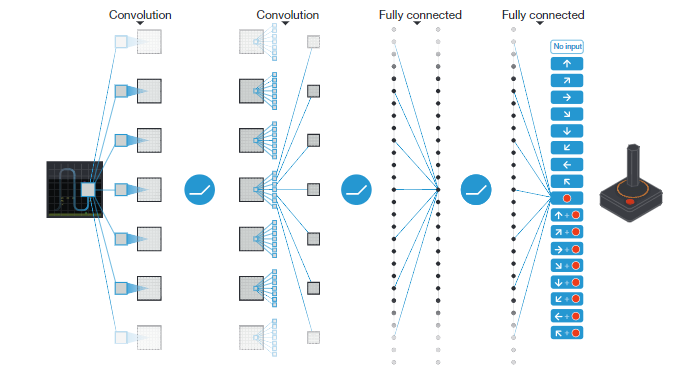
\includegraphics[scale=.85]{images/DQN-atari.png}
\caption{Deep Q-Network Architecture. The input consists of an 84x84x4 image. Each hidden layer is followed by a recitifier nonlinearity (max(0,x)).~\cite{atari}}
\label{fig:DQN-atari}
\end{figure}


\subsubsection{Experience Replay}

Experience replay is inspired by nature in the idea that learning a task can be learned better if an agent (human or animal) uses their past learnings.  Therefore, as the network is being trained experience data from the agent is stored in state-action-reward-nextState pairs ($<s,a,r,s^{*}>$). Batches of these experiences are drawn at random during training from an experience replay buffer which contains a set number of experiences.  As a new experience is learned it is added to the buffer and the oldest replay is removed. These batch experiences are used to update the weights of the network as the network navigates through a sequence of observations.  This allows the network to learn from a variety of past experience instead of finding a local minima in the immediate episode it is learning in~\cite{atari}.

\subsubsection{Seperate Target Network}

One main issue with Q-learning based reinforcement learning is that Q values are constantly shifted by small amounts during every iteration.  These constant shifts in values can cause a network to easily diverge, especially early on when the updates have a larger magnitude.  Using a seperate target network with Q values that is only updated periodically is one solution to this problem.  The network continues to update Q values iteratively, however, it will use the target network Q values in its calculations.  The target Q values are then updated periodically (adjustable hyperparameter) with the current calculated Q values in the network.  This gives the system stability, and removes tightly coupled correlations from influencing the network weights~\cite{atari}.


\subsection{Double Deep Q-Networks (DDQN)}

One set back found from using the traditional DQN~\cite{atari} is that it may overestimate Q values for certain actions in a state~\cite{van2016deep}. This poses a problem if Q values for actions were not overestimated equally which is usually the case.  Therefore, during training there is a high chance that some suboptimal actions may be given a high Q value early on which would cause the system to fall into a local minima.  Therefore Hasselt et al.~\cite{van2016deep} developed a technique called double DQN (DDQN) which utilized the network Q values and target-Q values.  In DQNs the max over Q values is used to compute the target-Q value, in double DQN the Q-values from the primary network are used to choose an action while the target-Q network is used to generate the target Q-value for the chosen action. Therefore, the action choice and target Q-value generation are decoupled which reduces overestimation and provides greater stability.  In~\cite{van2016deep}  the DDQN outperformed DQN on every Atari 2600 game except for two. The DDQN was also able to achieve super human level in games where DQN could not. 

\subsection{Dueling Deep Q-Networks (Dueling DQN)}
With the idea that Q-values directly correspond to how beneficial it is to take action ($a$) in a given state. Traditionally, this is used in this context, however Wang et al.~\cite{wang2015dueling} splits these Q-values into two seperate values.  One of the values is $V(s)$ which states how good it is to be in a given state. The second value is $A(a)$ which is the advantage function stating the advantage of taking action $a$ compared to the other possible actions.  Therefore, Q is decomposed as show in (\ref{eq:duelingQ})~\cite{wang2015dueling}.

\begin{equation}
          \label{eq:duelingQ}
          \resizebox{0.4\textwidth}{!}{$Q(s,a) = V(s) + A(a)$}~\cite{wang2015dueling}%
\end{equation}
Therefore, dueling DQNs contain two networks, one to compute $V(s)$ and one to compute $A(a)$.  The outputs of these networks are then combined to find the final Q-value ($Q(s,a)$) as shown in Fig.~\ref{fig:duelingDQN}~\cite{wang2015dueling}.

\begin{figure}
\centering
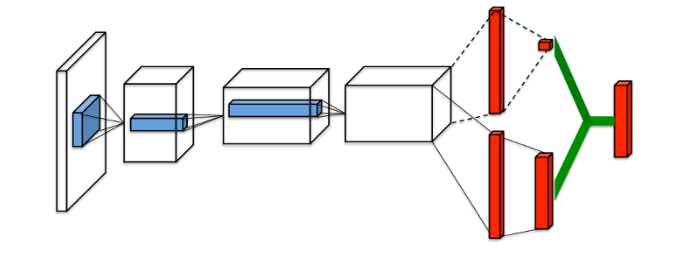
\includegraphics[scale=.85]{images/duelingDQN.png}
\caption{Dueling Deep Q-Network Architecture. Two networks are used and combined at the end.~\cite{wang2015dueling}}
\label{fig:duelingDQN}
\end{figure}

The idea of seperating Q-values into these two value functions is to be able to create robust state value estimates without having it to be attached to a specific action.  For example, consider an agent in a room where it recieves a very high reward of being in the green zone and a very low reward of being in the red zone. If the agent is in the green zone it is highly rewarding to be in that zone, and no action needs to be taken to recieve reward. Therefore, it does not make sense in this case to consider the value of being in the green zone state being coupled with an action. Therefore, by decoupling the value of being in a state and the advantage of taking an action more complex and robust estimates can be made that allow for greater stability and faster learning~\cite{wang2015dueling}. This paper~\cite{wang2015dueling} also used Atari 2600 as its bench mark and greatly outperformed both DDQN and DQN architectures. 

\subsection{Deep Recurrent Q-Networks (DRQN)}
In DQNs~\cite{atari}, DDQNs~\cite{van2016deep}, and Dueling DQNs~\cite{wang2015dueling} allow the agent to have full access to the information of the environment. In other words, our system has full observability in that it is given full state information of the entire game state.  For example, grid worlds and Atari 2600 games have all the information of the world in a single state (no scrolling game play or worlds). However most real world problems will not give an agent full observability. Assume an agent does not have access to all the information in a world (partial observability), traditional DQN methods will not be able to converge. For example, in cases where there are walls or doors an agent will not know the states that are on the otherside. Also, while spatial limitations exist, temporal information is also crucial.  Often, in single image inputs motion, speed, and direction can be lost to an agent. Even in DQN architectures, only 4 frames are used as an input, therefore in environments where past information is even more crucial these 4 frames greatly limit what can be learned. Enviroments where all information is not available to an agent are called Partially Observable Markov Decision Processes (POMDPs).  

Hausknecht et al.~\cite{HausknechtDRQN} found that the performance of DQNs decline when trying to learn a POMDP and could be better learned using recurrent neural networks. This created the Deep Recurrent Q-Network (DRQN) architecture. Instead of passing in a series of images as input to the network, DRQNs take in a single image. The difference lies in the first fully-connected layer being replaced with a recurrent LSTM layer. This change can be seen in Fig.~\ref{fig:drqn-arch}~\cite{HausknechtDRQN}.

\begin{figure}
\centering
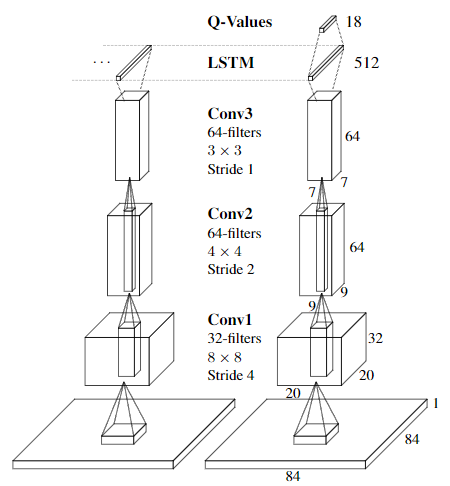
\includegraphics[scale=.85]{images/drqn-arch.png}
\caption{DRQN Architecture~\cite{HausknechtDRQN}.}
\label{fig:drqn-arch}
\end{figure}

As shown, the LSTM layer is instered just before the value and advantage layers are calculated the same as in dueling DRQNs. Another change in this network is in the experience replay.  Instead of selecting a random batch of experiences, DRQNs train on random batches of sequence of experiences at a set length.  This is important so that sequences can be learned which is crucial to the recurrent nature of DRQNs. Using this network with the Atari 2600 framework, DRQNs showed significant improvement on POMDP style game play~\cite{HausknechtDRQN}. 


\section{Examples}


\chapter{Deep Inverse Reinforcement Learning}
TODO: WRITE GENERAL INTRODUCTION
\section{Related Work}
\label{sec:maxentdeepirl}
\subsection{Deep Maximum Entropy IRL}
Wulfmeier et al.~\cite{wulfmeier2015maximum} used multi-layer neural networks to implement Section~\ref{sec:maxentirl} without the need to hand-craft features. Using similar gridded environments as~\cite{ziebart2008maximum}, a neural network (specifically a Fully Convolutional Neural Network) with wide convolutional layers (width one) is used to learn spatial features based on raw input.  

The first tests of this network used a regular neural network structure without any convolution layers, therefore the inputs were expert trajectories. The output of this neural network is used to estimate the reward function as is done in traditional inverse reinforcement algorithms. The input of this network is expert demonstrations ($\mu_{D}^{a}$) of state ($s$), action ($a$), reward pairing. The high level algorithm deals with iterating over \textit{n} epochs which represent the amount of gradient descent iterations. First, randomly intialized weights ($\alpha$) are forward propagated in the neural network.  The reward ($r^n$) is then extracted from this model and used to find an approximate policy ($\pi^n$) using value iteration. This policy is then used to find the expected state visitation frequency ($E|\mu^n|$) for each state (\textit{s}) as defined in Section~\ref{sec:maxentirl}.  The maximum entropy loss is found by (\ref{eq:maximum_entropy_loss}) using maximum entropy theory. The gradient is computed by taking the gradient of (\ref{eq:maximum_entropy_loss}) with respect to the reward ($r^n$) which is equivalent to the difference of the expected state visitation frequency of the expert ($\mu_D$) and learner expected state visitation frequency ($E|\mu^n|$) as shown in (\ref{eq:maximum_entropy_gradient}).  This is the same gradient calculation as found in~\cite{ziebart2008maximum}.  This gradient is then backpropagated through the network to update nodes.  The weights ($\alpha$) are then also updated with this gradient and the algorithm repeats until the number of epochs is reached. 

\begin{equation}
            \label{eq:maximum_entropy_loss}
            \resizebox{0.3\textwidth}{!}{$L_{D}^{n}=log(\pi^n) \times \mu_{D}^{a} $}~\cite{wulfmeier2015maximum}% 
        \end{equation}

\begin{equation}
            \label{eq:maximum_entropy_gradient}
            \resizebox{0.3\textwidth}{!}{$\frac{\delta L_{D}^{n}}{\delta r^{n}}=\mu_D -  E|\mu^n|$}~\cite{wulfmeier2015maximum}% 
        \end{equation}

This paper implemented and analyzed their DeepIRL solution on two types of environments, Objectworld and Binaryworld. An objectworld consists of an $M$x$M$ grid representing $M^2$ possible states.  There are 4 possible actions for an agent to move (up, down, left, right, stay in place). The state features are defined as the minimum distance to colored object.  The objects can be one of $C$ colors. The reward is defined as positive for grid cells which are distance 3 of color 1 and distance 2 of color 2. The reward is defined as negative for grid cells which are only within distance 3 of color 1, and zero otherwise.  The binaryworld consists of states being randomly assigned blue or red.  The feature vector for each state is a binary vector of length 9 which encoded the color of each cell in a 3x3 neighborhood. The reward is positive if 4 out of 9 neighboring states are blue, negative if exactly 5 are blue, and zero otherwise.  The binary world relies on a direct relationship between states which makes it a unique, and complex problem to solve. For both worlds the DeepIRL network produced state of the art results, however, inclusion of convolutional layers (Fully Convolutional Neural Network [FCNN] with width one) allows for the input of raw input without the need of hand-crafted features (such as what is needed for objectworld and binaryworld). The raw input is the entire state-space with what each state occupies (objects for objectworld, color for binaryworld). This allows the network to not only learn an appropriate reward function but also spatial features of the input environment in terms of the expert trajectory data.  One drawback of this is that more expert samples are needed for training to match performance of DeepIRL network without a CNN, however, this extends this architecture to take in raw image data to learn complex tasks in complex environments~\cite{wulfmeier2015maximum}.

\section{Examples}

\chapter{Platform}
Generally environments that make use of automatic guided vehicles (AGVs) have to plan the path(s) where the robots should go before installing the tracks, like magnetic strips or metal tracks; this is an investment even before using the robots. If any change to the path(s) is required to be made, then more cost is incurred. For this research a four wheeled differential drive robot has been controlled wirelessly to follow paths drawn on a graphical user interface within a workspace of 1.8m by 1.4m. The robot is controlled by correcting its orientation through visual feedback from a camera. Error analysis was performed to investigate how well the robot followed the path drawn. The estimated error of the robot is within a few centimeters of the path and can be reduced by modifying various thresholds.

\section{Background}
Robots whose path is controlled by the user are termed as automatic guided vehicles (AGVs). AGVs follow paths using lasers, cameras, or are physically attached to these paths. These mobile robots follow predefined routes and so, are heavily used in industries for materials handling. Apart from transporting loads, these kinds of robots are used in risky environments and explorations, like space, mines and underwater. For guiding some AGVs, lines, magnetic tracts, or wires are installed on warehouse floors. Hence, making use of these robots requires an initial investment. Vision-based AGVs follow a physical line or markers in a room: landmark based navigation.  Combining these ideas a robotic system was created for dynamic path following using vision based control.  

This research platform uses a wireless automatic guided robot that does not require any kind of intrusive modifications to be made to the environment apart from installing an overhead camera. The camera above the workspace tracks the robot continuously and is used to help correct it to follow a predefined path. The user is allowed to define the path the robot should follow in a GUI created in MATLAB.

Using a live image of the environment from a bird's-eye-view, the robot is tracked in real-time using ArUco fiducial markers.  The live images are fed to a software GUI where the user can freehand draw any path they desire directly on top of the image.  The system then sends commands to the robot to move it along this path by using the camera and ArUco markers as feedback control. Doing this, the user can draw complicated paths around a room and around obstacles for the robot to navigate. 

\section{System Overview}
This system consisted of four main sub-components; the Robot, OpenCV, MATLAB, and the Environment workspace itself. Fig.~\ref{fig:workflow} shows the entire system architecture and work flow using these four main components.
\begin{figure}[h!]
\centering
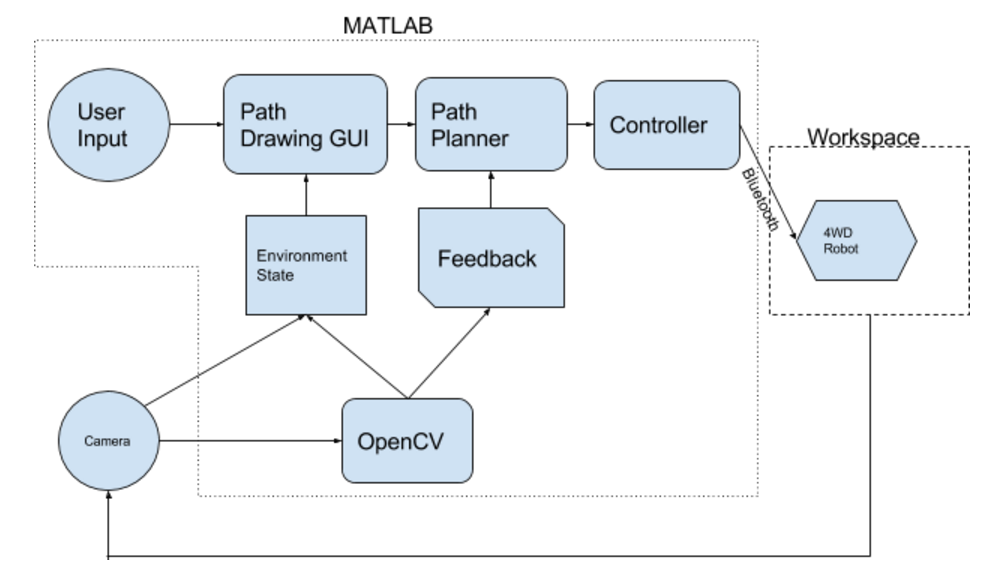
\includegraphics[scale=.5]{images/workflow.PNG}
\caption{System Work Flow}
\label{fig:workflow}
\end{figure}

\subsection{Differential Wheel Drive Robot}
Four-wheeled differential drive robotics platforms are commonly used in navigation applications. The system used in this setup was the 4WD Rover I from Lynxmotion, as shown in Fig.~\ref{fig:robot}.

\begin{figure}[h!]
\centering
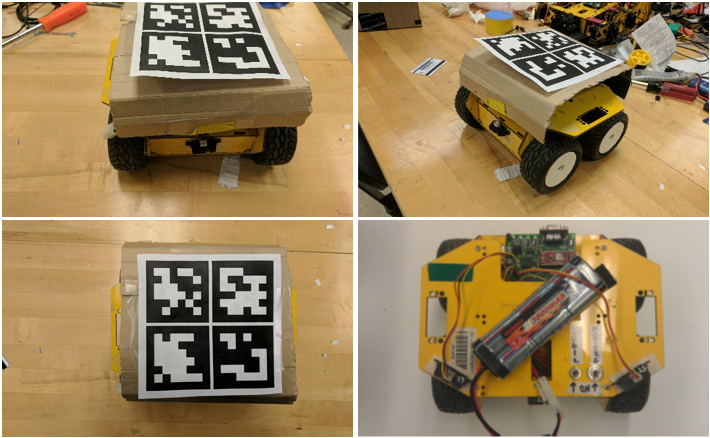
\includegraphics[scale=.5]{images/robot.PNG}
\caption{4WD Rover I from Lynxmotion}
\label{fig:robot}
\end{figure}

In this type of system each pair of wheels can be controlled independently from another pair.
Therefore, this allows the robot to rotate about its center, which gives it greater control and speed on
sharp angled turns. To control these motors, pulse width modulation (PWM) signals are given to each motor. This type of signal is usually at a fixed frequency and is a digital square wave ranging from 0V to \textit{$V_{max}$}. \textit{$V_{max}$} for the specific application performed was 7.2V. The signal determines on and off time for the motor based on its duty cycle. A duty cycle of 50\% will result in the motors being powered at half their capacity. A duty cycle of 10\% will result in the motors being powered at a tenth of their capacity. A duty cycle of 100\% will result in the motors being powered at full capacity
which looks like a DC signal at 7.2V. These duty cycles are shown in Fig~\ref{fig:pwm}. To control the duty cycle, an Arduino Uno was used which is the main controller used for the four-wheeled robot. A value of 0 to 255 was
used to set the duty cycle between 0 and 100\%. In this case 0 would represent 0\% or full stop, 128 would represent 50\% or half speed, and 255
would represent 100\% or full speed.
\begin{figure}[h!]
\centering
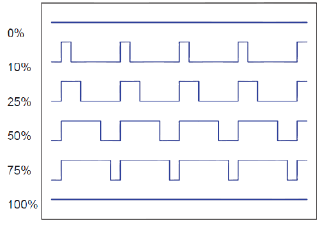
\includegraphics[scale=1]{images/PWM.PNG}
\caption{Various duty cycles on PWM signals}
\label{fig:pwm}
\end{figure}

This robot was programmed through the Arduino to take in serial commands to determine motion.  Single character commands were used as shown in Table~\ref{tab:movement}. To take in these serial commands, a Bluetooth module was connected to the Arduino's TX and RX lines.  The module used was the HC-06, which is a low-power slave Bluetooth module. Once the Arduino receives a movement command it sends the appropriate PWM signals to the Pololu Dual MC3926 motor controller board which was wired
directly to the motors, battery, and Arduino Uno. 
\begin{table}[h!]
\centering
\caption{Movement Commands}
\label{tab:movement}
\begin{tabular}{|p{1.5cm}|p{1cm}|p{3cm}|}
\hline
\textbf{Command} & \textbf{Function} & \textbf{Wheel Movement} \\ \hline
F & Move Forward & All wheels turn in same direction, forward \\ \hline
L & Turn Left & Left side wheels reverse, right side wheels forward \\ \hline
R & Turn Right & Right side wheels forward, left side wheels reverse \\ \hline
S & Stop & Duty cycle of all wheels set to 0\%, no movement \\ \hline
\end{tabular}
\end{table}

\subsection{OpenCV}

OpenCV is a comprehensive computer vision toolbox used for a variety of real-time applications such as tracking, facial recognition, segmentation, and classification. It is originally written in C++ but wrappers have been made to allow it to be used in Python and MATLAB. For this system, the only component of OpenCV being used is video stream capture and the ArUco Marker detection.  ArUco markers are pattern-based black and white squares that can be easily identified through OpenCV.  Since OpenCV knows what patterns to look for, it can identify ArUco markers in an environment and determine the corners of them as well as the orientation. For this application four ArUco markers were used as shown in Fig.~\ref{fig:ArUco}. This marker array was printed to the size 14.5 cm by 14.5 cm and was  mounted flat on top of the robot so that the center of the array was at the center of the robot.  The top two markers were facing in the direction of the front of the robot and were used as a reference to determine the orientation of the robot.

\begin{figure}[h!]
\centering
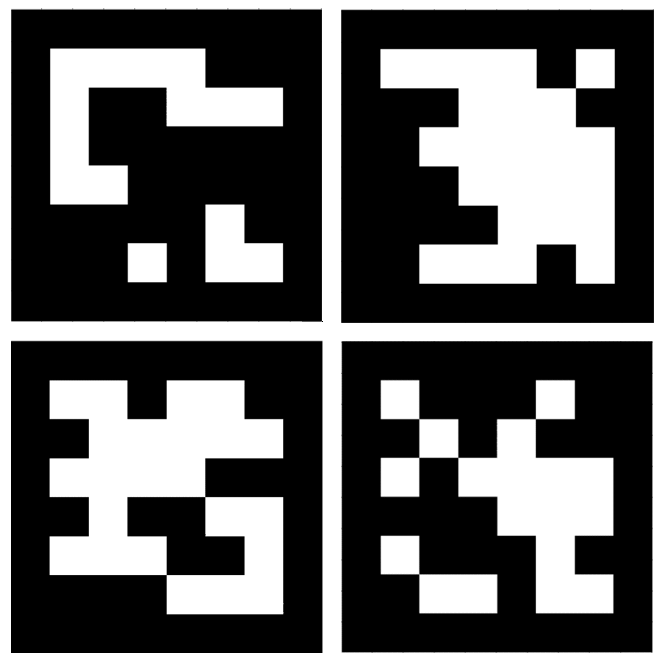
\includegraphics[scale=.45]{images/ArucoArray.PNG}
\caption{ArUco Array of four markers}
\label{fig:ArUco}
\end{figure}

\subsection{MATLAB}

MATLAB is a powerful computing platform.  It uses a scripting based language which is ideal for fast prototyping.  It has also been built to be computationally efficient especially in terms of matrix math and neural networks. In this system, MATLAB is used to create the main GUI, interface with OpenCV, interface with the camera, path creation and planning, and sending serial commands to the robot via Bluetooth.  

\subsection{Environment}

The environment that the robot resides in can be variable.  However, the surface on which the robot roams needs to be navigable by the robot chassis. Also, the environment needs to be well lit so that the markers can be detected. A webcam was placed on the ceiling of the room which was about 8 feet from the ground and faced perpendicular to the floor. The webcam used is shown in Fig.~\ref{fig:webcam}. The webcam itself was used with a resolution of 640 px by 480 px.  This created view-able workspace of about 1.8m (6 feet) by 1.4m (4.5 feet). The robot was placed within this static workspace. The webcam was connected to the computer running the MATLAB application through USB.

\begin{figure}[h!]
\centering
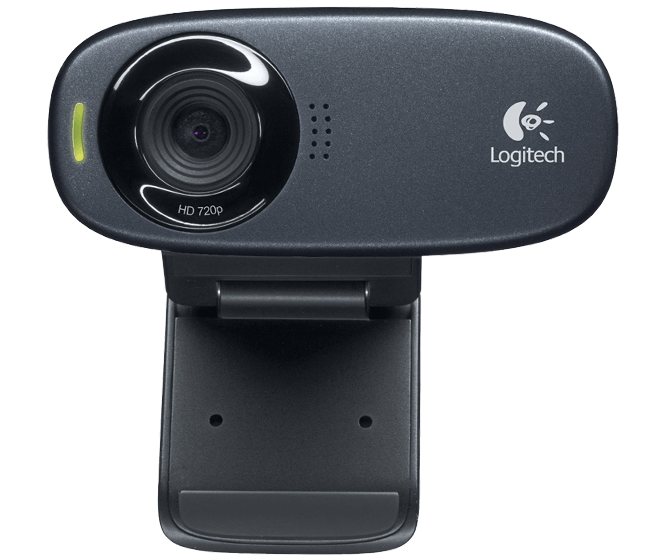
\includegraphics[scale=.15]{images/webcam.png}
\caption{Webcam used for tracking}
\label{fig:webcam}
\end{figure}

\section{Procedure}
As an overview, the procedure of running this system takes into account all four main components.  First, the camera is set-up to view a bird's-eye view of the workspace.  The robot is then placed within that workspace with its ArUco markers. The application is then started using MATLAB. OpenCV functions are used to detect the ArUco markers and determine the millimeter to pixel ratio since the ArUco markers are a known size. Once the robot is detected the user is prompted to draw a path over the current image. This path is then fed to the path planner code where the robot iteratively follows the following steps:
\begin{itemize}
\item The robot faces desired point
\item The robot goes towards point
\item Feedback from OpenCV to determine whether or not robot meets success thresholds
\item The robot's movement is adjusted to meet threshold if needed
\item Once the point is reached, the desired point moves to the next point
\end{itemize}
Once the robot completes the desired path the errors from the robot movement versus the ground truth path are found.  The user is then prompted to draw another path. This basic procedure is shown in the flowchart in Fig~\ref{fig:flowchart}.

\begin{figure}[h!]
\centering
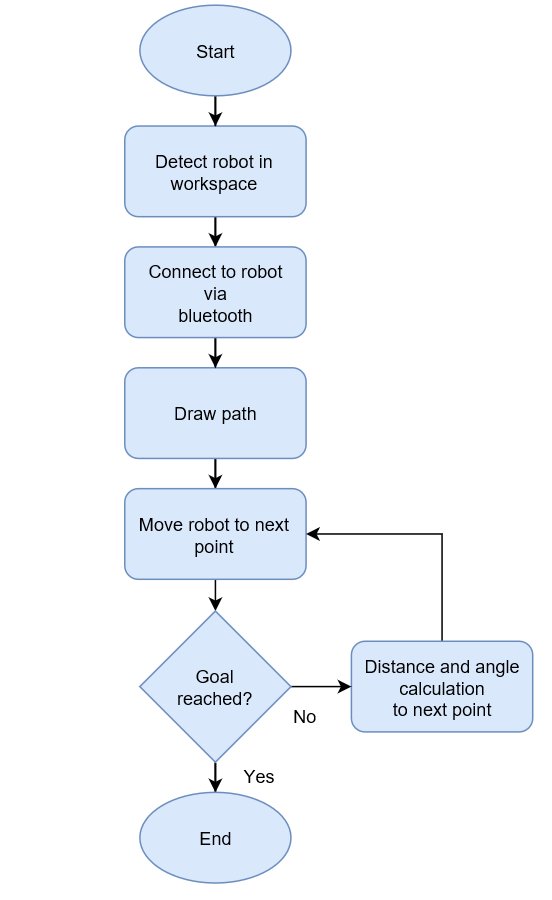
\includegraphics[scale=.5]{images/flowchart.PNG}
\caption{Basic Flowchart of Procedure}
\label{fig:flowchart}
\end{figure}


\subsection{Detecting ArUco Markers} 

To detect the 4 ArUco markers on the robot, the ArUco marker library within OpenCV was used. This library contains a function \textit{detectMarkers} which takes in an image (that contains the markers), a dictionary of marker definitions, and some optional parameters. It then returns the corner locations and ID numbers for all markers detected.  Once the corners and IDs are found, as shown in Fig.~\ref{fig:ArUcodetected}, the center point for the array is also found.  
\begin{figure}[h!]
\centering
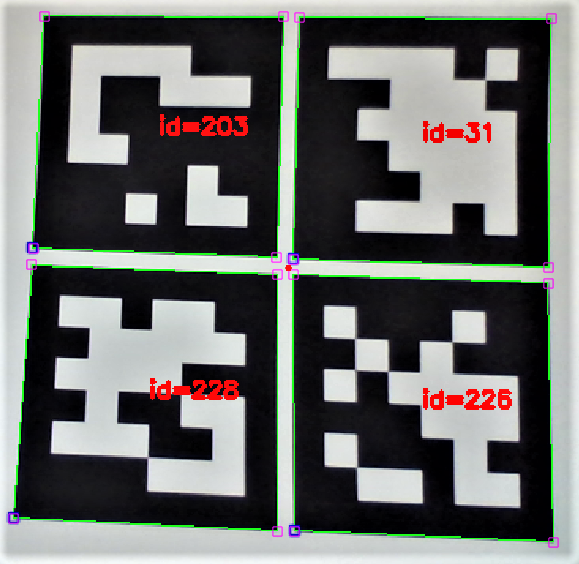
\includegraphics[scale=.5]{images/ArucoDetected.PNG}
\caption{Annotated ArUco Array of four markers}
\label{fig:ArUcodetected}
\end{figure}
This is done by using a centroid function that uses the points of the 4 corners closest to the center of the image.  This is shown in Equation~\ref{eqn:centerx} and~\ref{eqn:centery} where n is equal to 4 to represent the four points used.  This center point is used to determine the center of the robot, which is also its turning axis. 
\begin{equation}
center_x = \frac{\sum_{k=0}^{n}{x_k}}{n}
\label{eqn:centerx}
\end{equation}
\begin{equation}
center_y = \frac{\sum_{k=0}^{n}{y_k}}{n}
\label{eqn:centery}
\end{equation}

\subsection{Drawing a Path}

Once the robot and the markers are detected in the frame of the workspace the user is prompted to draw a path.  This is done by using the built in \textit{imfreehand} function on the current image of the workspace.  This allows the user to freely drawing any path within the workspace as shown in Fig.~\ref{fig:pathdrawn}.
\begin{figure}[h!]
\centering
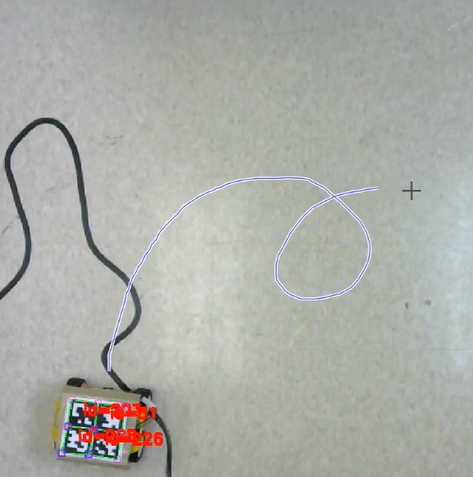
\includegraphics[scale=.5]{images/pathDrawn.PNG}
\caption{Path Drawn by user in GUI}
\label{fig:pathdrawn}
\end{figure}
 Once the user draws the path the path is represented by a solid red line with a white star at its first point and a yellow star at its end point.

\subsection{Accuracy Thresholds}

To ensure the robot follows the path accurately, thresholds were created for the allowable distance it was from the desired point and its orientation with respect to the next point. To identify the distance in pixels between the desired point and the robot, denoted as \textit{d}, the euclidean distance between the desired point and the center point of the ArUco marker array was found. This equation is shown in \ref{eqn:distance}, where $x_c$ and $y_c$ are the pixel coordinates for the center of the robot, and $x_g$ and $y_g$ are the pixel coordinates for the desired point (current point on path trying to be reached). If the value of \textit{d} was less than the threshold (by default was 20 pixels) then the robot met the distance criteria.

\begin{equation}
d = \sqrt[]{(x_c - x_g)^2 + (y_c - y_g)^2}
\label{eqn:distance}
\end{equation}

The second criteria was the orientation of the robot to the next point. This was important to meet so that the robot was always following the trajectory of the path. To do this 3 vectors were found and plotted. The first vector was from the center of the robot to the desired point ($V_g$). The second vector was from the center of the robot to the front of the robot between ArUco markers 31 and 203 ($V_o$). The third vector was from the front of the robot to the desired point ($V_n$). These vectors are shown in Fig.~\ref{fig:orientation}.

\begin{figure}[h!]
\centering
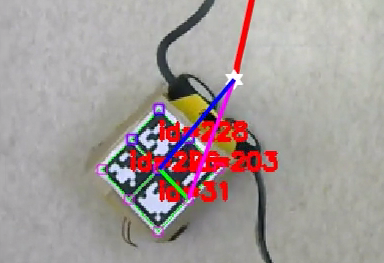
\includegraphics[scale=1]{images/angle.PNG}
\caption{Setting Robot Heading Direction: white star indicates desired point; green indicates current heading direction between center and front of robot ($V_o$); blue indicates desired heading direction between center and desired point ($V_g$); magenta indicates difference between the directions which is the vector from the front of the robot to the desired point ($V_n$)}
\label{fig:orientation}
\end{figure}

To use these vectors to modify the robot's current heading, they were first normalized by dividing the vector elements ($x$ and $y$) by the magnitude of the vector. The dot product was then taken between $V_o$ and $V_g$ as shown in Equation~\ref{eqn:orientation}. Where $a$ is a value between 1 and -1. The desired orientation value of the robot is 1 which means that the robot's heading is facing towards (parallel) the desired point.  At -1, the robot is facing the opposite way of the desired point. An orientation threshold was defined to be close to 1 to make the robot more accurate in path following.
\begin{equation}
a = V_o  \bm{\cdot} V_g
\label{eqn:orientation}
\end{equation}

The $a$ value gives us information on heading but does not tell the optimal way for the robot to turn. The system could have been setup to turn left every time the heading was less than the threshold until the orientation threshold was met, but that would not be optimal.  To determine the direction the robot should turn to make the most optimal decision to meet the orientation threshold Equation~\ref{eqn:theta} is used. Where the two parameters of the \textit{atan2} function are the \textit{sin($\theta$)} and \textit{cos($\theta$)}.  This function returns the four quadrant inverse tangent that will give a $\theta$ value between 180$\degree$ and -180$\degree$.  This gives us the exact angle between the $V_g$ and $V_n$ vectors to determine which direction to turn.  Since this angle is in reference to the current heading of the robot, a positive $\theta$ value will mean that the robot needs to turn left, and a negative $\theta$ value will mean that the robot needs to turn right. 
\begin{equation}
\theta = atan2(V_{g_{x}}*V_{n_{y}}-V_{g_{y}}*V_{n_{x}}, V_{g_{x}}*V_{n_{x}}+V_{g_{y}}*V_{n_{y}}) 
\label{eqn:theta}
\end{equation}

Therefore, using the values $d$, $a$, and $\theta$ the robot's movement is altered using Algorithm~\ref{alg:movement}. To ensure that the robot has enough time to act before another command is sent to it the movement commands were only sent once a certain time threshold was met. Therefore, some movement commands were skipped to allow the robot's movement to be smooth and to ensure that the serial buffer on the robot would not be overflown. 
\begin{algorithm}
\caption{Robot Next Move}
\label{alg:movement}
\begin{algorithmic} 
\If{$d < distanceThreshold \land a > orientationThreshold$}
\State $desiredPoint \leftarrow nextPoint$
\ElsIf{$a < orientationThreshold$}
\If{$\theta > 0$}
\State $Turn Left$
\Else
\State $Turn Right$
\EndIf
\ElsIf{$d > distanceThreshold$}
\State $Move Forward$
\EndIf
\end{algorithmic}
\end{algorithm}


\subsection{Following the Path} 

Using Algorithm~\ref{alg:movement}, the robot went to each point on the path drawn by the user. As it did this, the center point of the robot was plotted every time a point was reached. Using this data the, the overall error of the physical robot path was determined. Fig.~\ref{fig:pathfollowing} shows a snapshot of a robot following a path. 

\begin{figure}[h!]
\centering
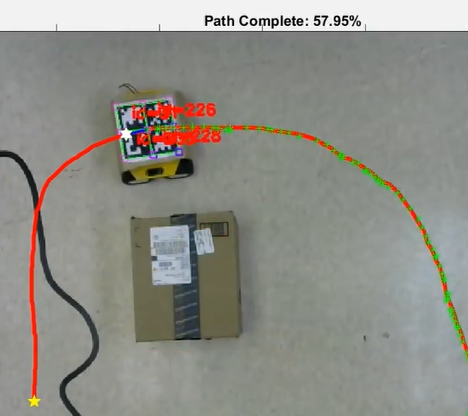
\includegraphics[scale=.5]{images/star.PNG}
\caption{Robot following the Path: white star indicates next point to reach; green markings show robot's past positions, yellow star indicates goal}
\label{fig:pathfollowing}
\end{figure}

\subsection{Accuracy Analysis}
To determine the overall accuracy of the robot, error between the physical path the robot took and the actual path was measured. This accuracy was improved by changing the distance and orientation thresholds for the system. At the end of each path taken, the error magnitude for each point is displayed as well as the standard deviation of error, mean error, maximum error, minimum error, and estimated error. The estimated error is defined as the error that will be found 95\% of the time or two standard deviations ($\sigma$) away from the mean ($\mu$), as shown in Equation~\ref{eqn:esterror}. 

\begin{equation}
Est. Error = \mu + 2*\sigma 
\label{eqn:esterror}
\end{equation}

Three trials were tested with varying threshold values.  Fig.~\ref{fig:results1},~\ref{fig:results2}, and~\ref{fig:results3} show several paths with their corresponding error charts.

\begin{figure}[h!]
\centering
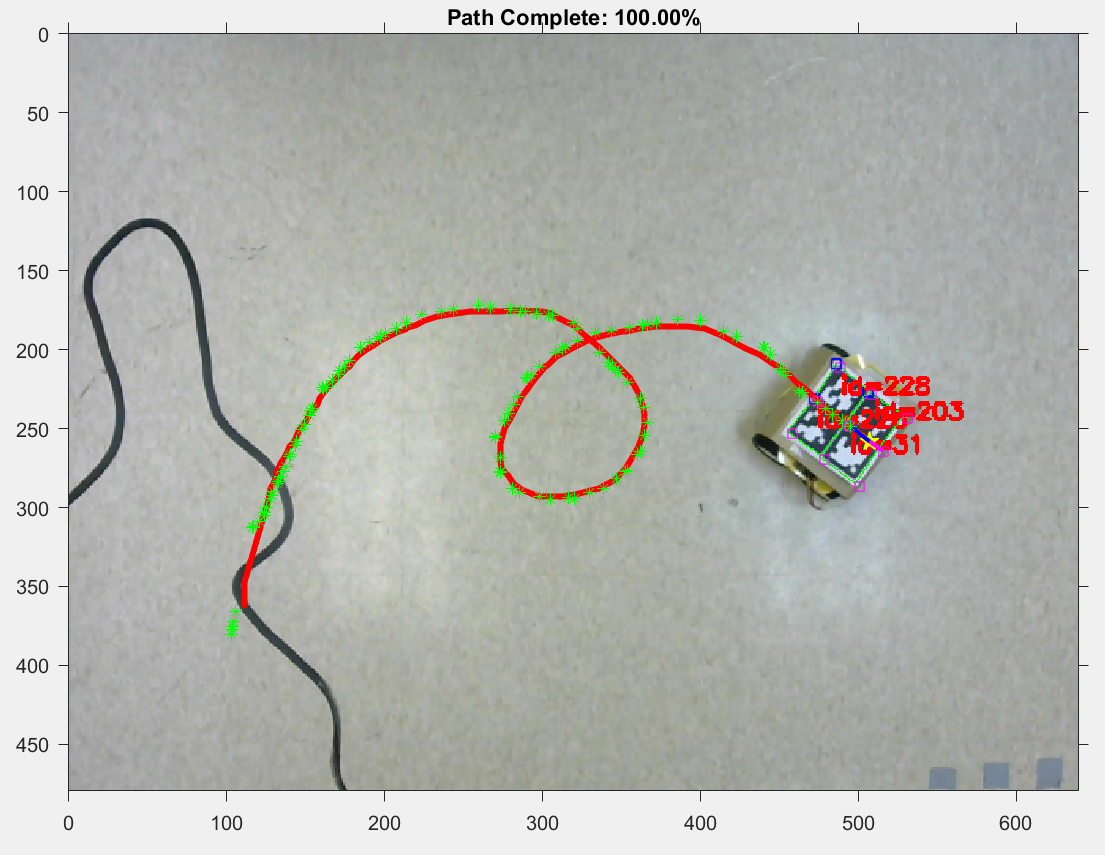
\includegraphics[scale=.25]{images/PATH-2095-1.PNG}
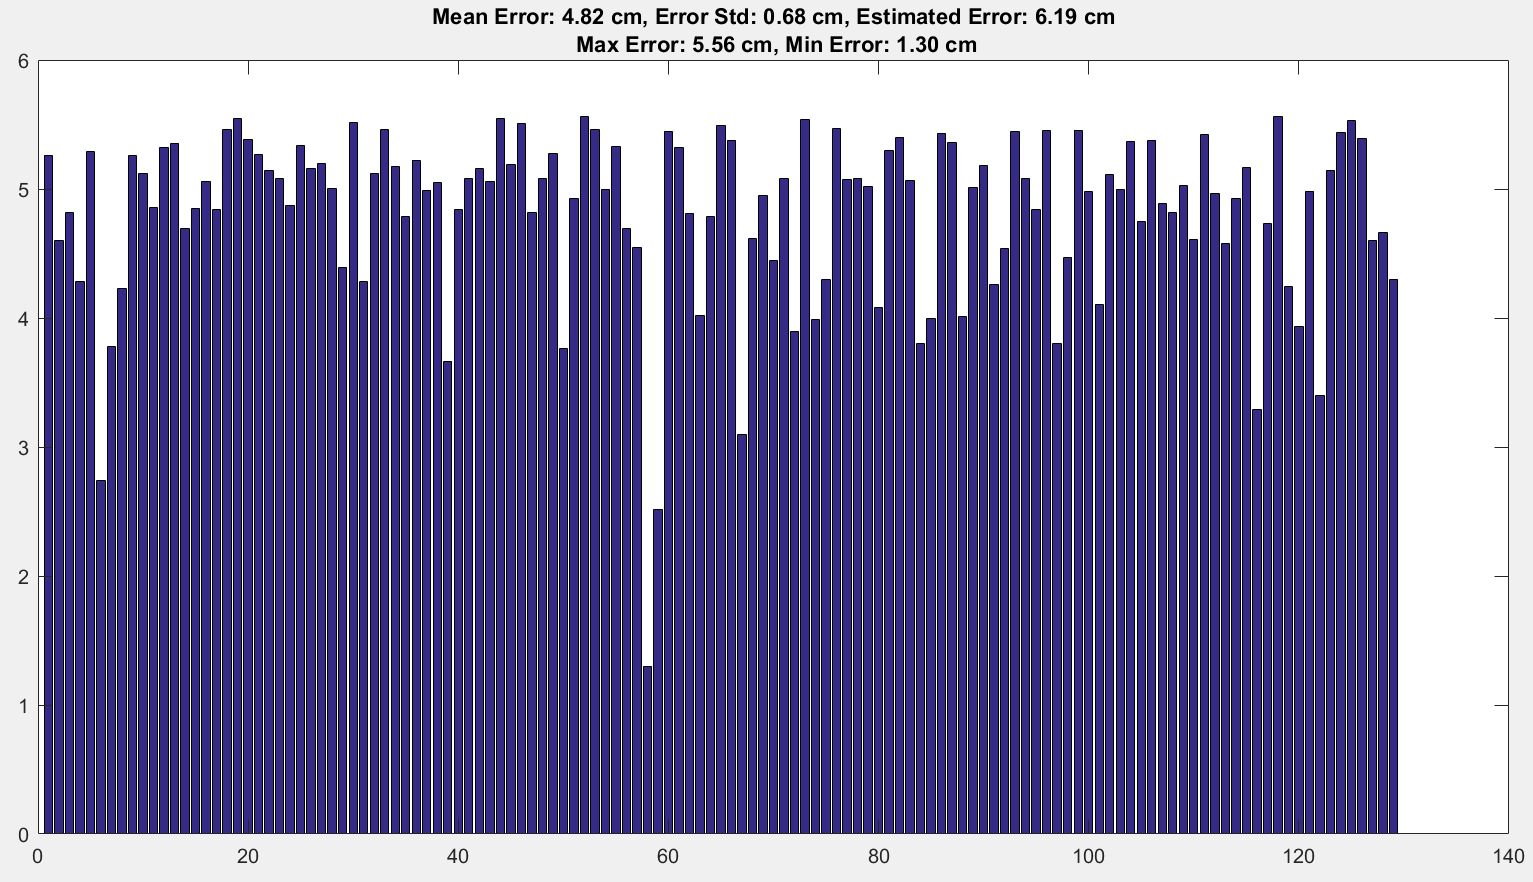
\includegraphics[scale=.25]{images/DATA-2095-1.PNG}
\caption{Results for robot motion with distanceThreshold = 20px and orientationThreshold = 0.95}
\label{fig:results1}
\end{figure}

\begin{figure}[h!]
\centering
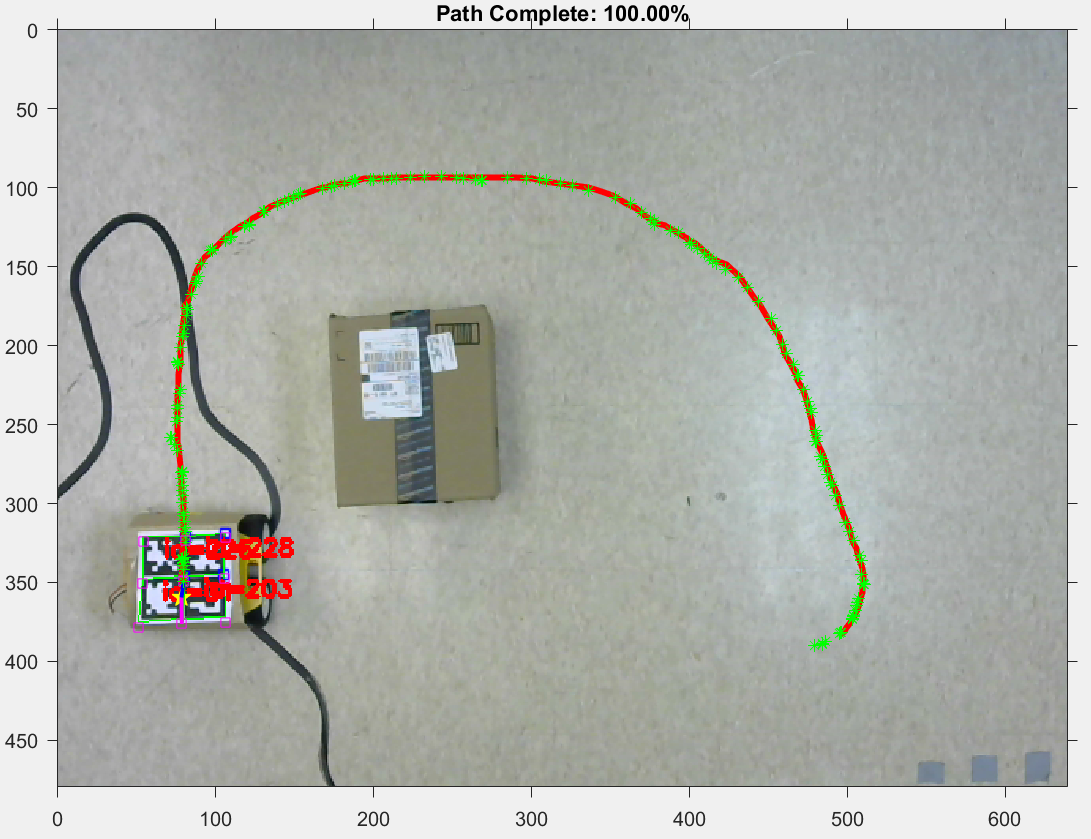
\includegraphics[scale=.25]{images/PATH-2099.PNG}
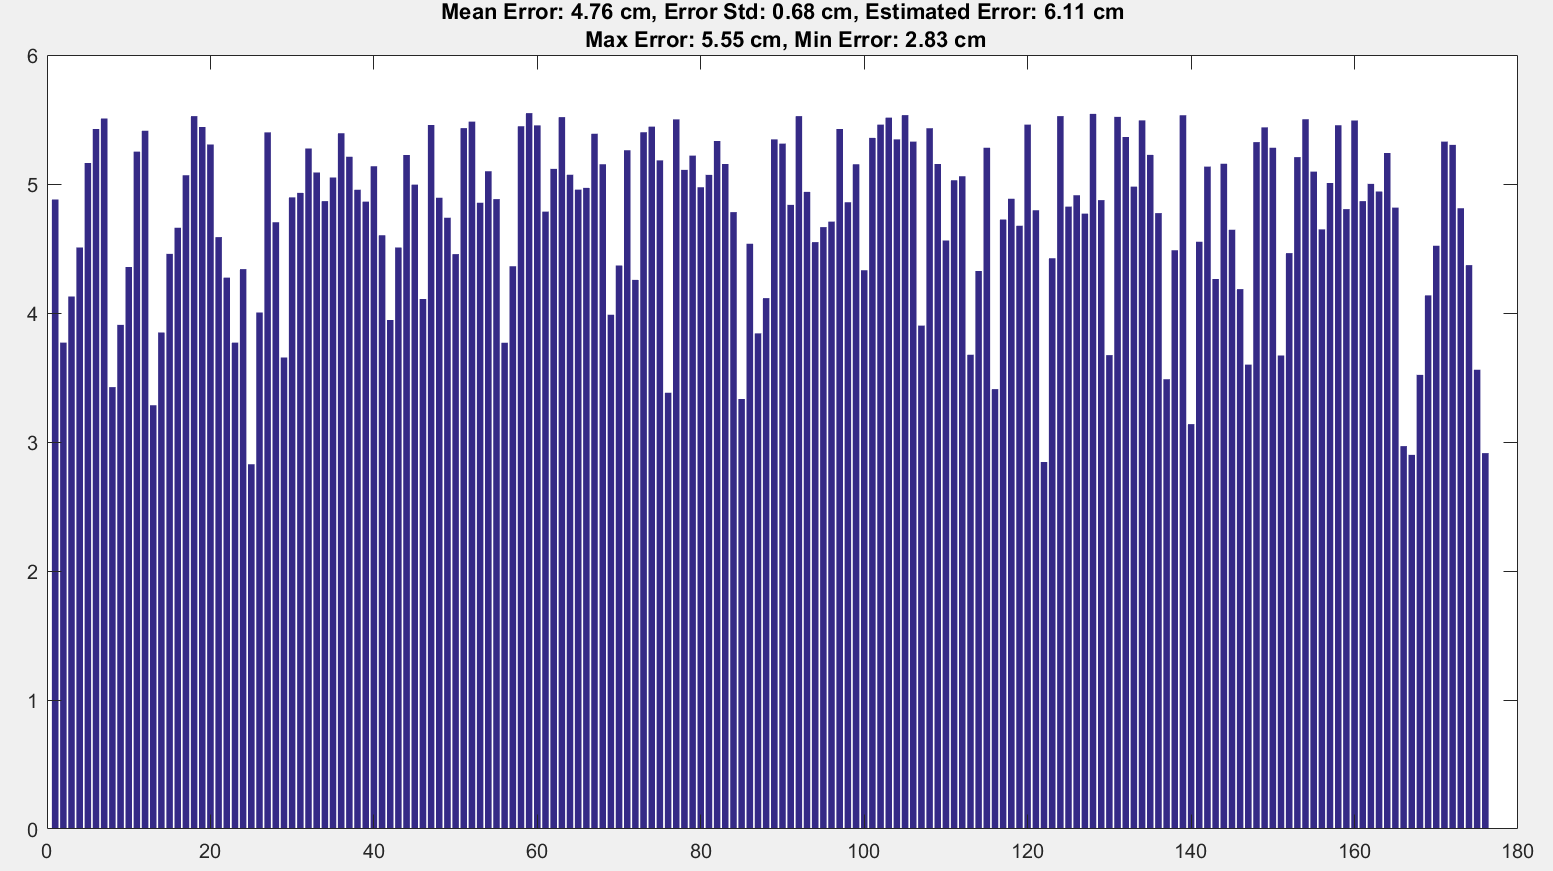
\includegraphics[scale=.25]{images/DATA-2099.PNG}
\caption{Results for robot motion with distanceThreshold = 20px and orientationThreshold = 0.99}
\label{fig:results2}
\end{figure}

\begin{figure}[h!]
\centering
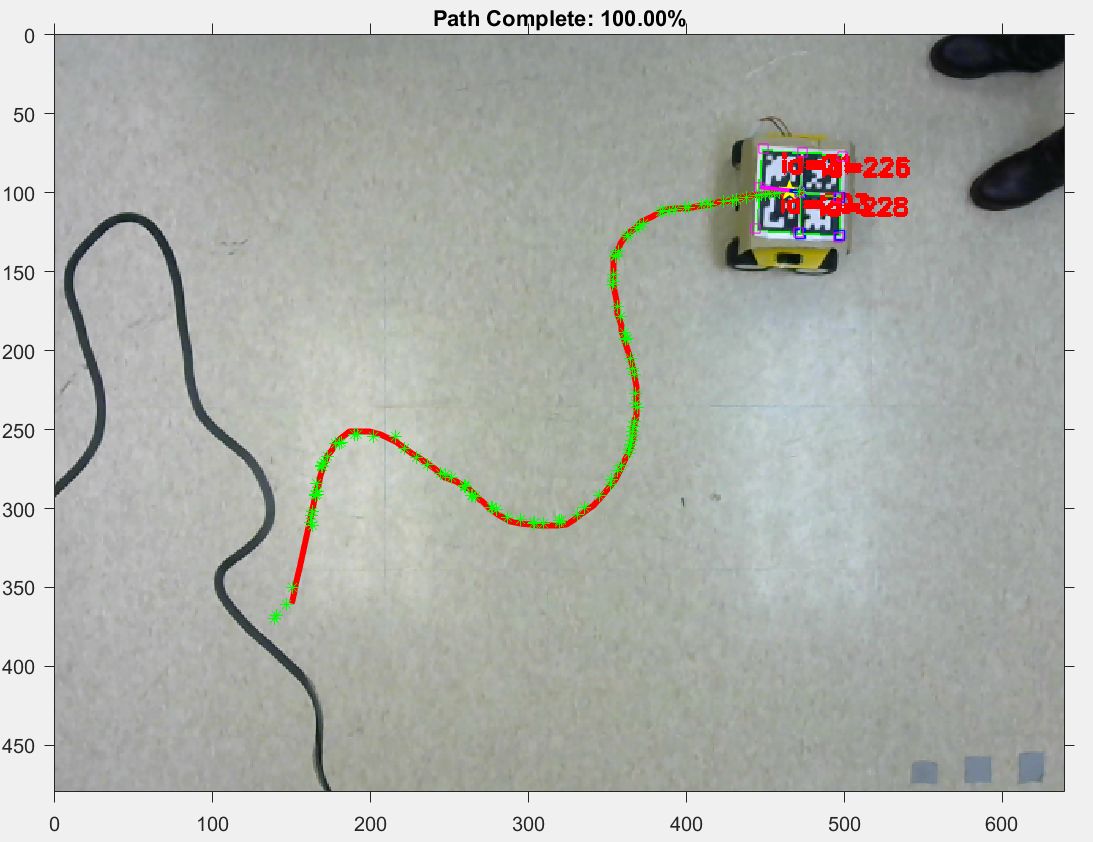
\includegraphics[scale=.25]{images/PATH-1599.PNG}
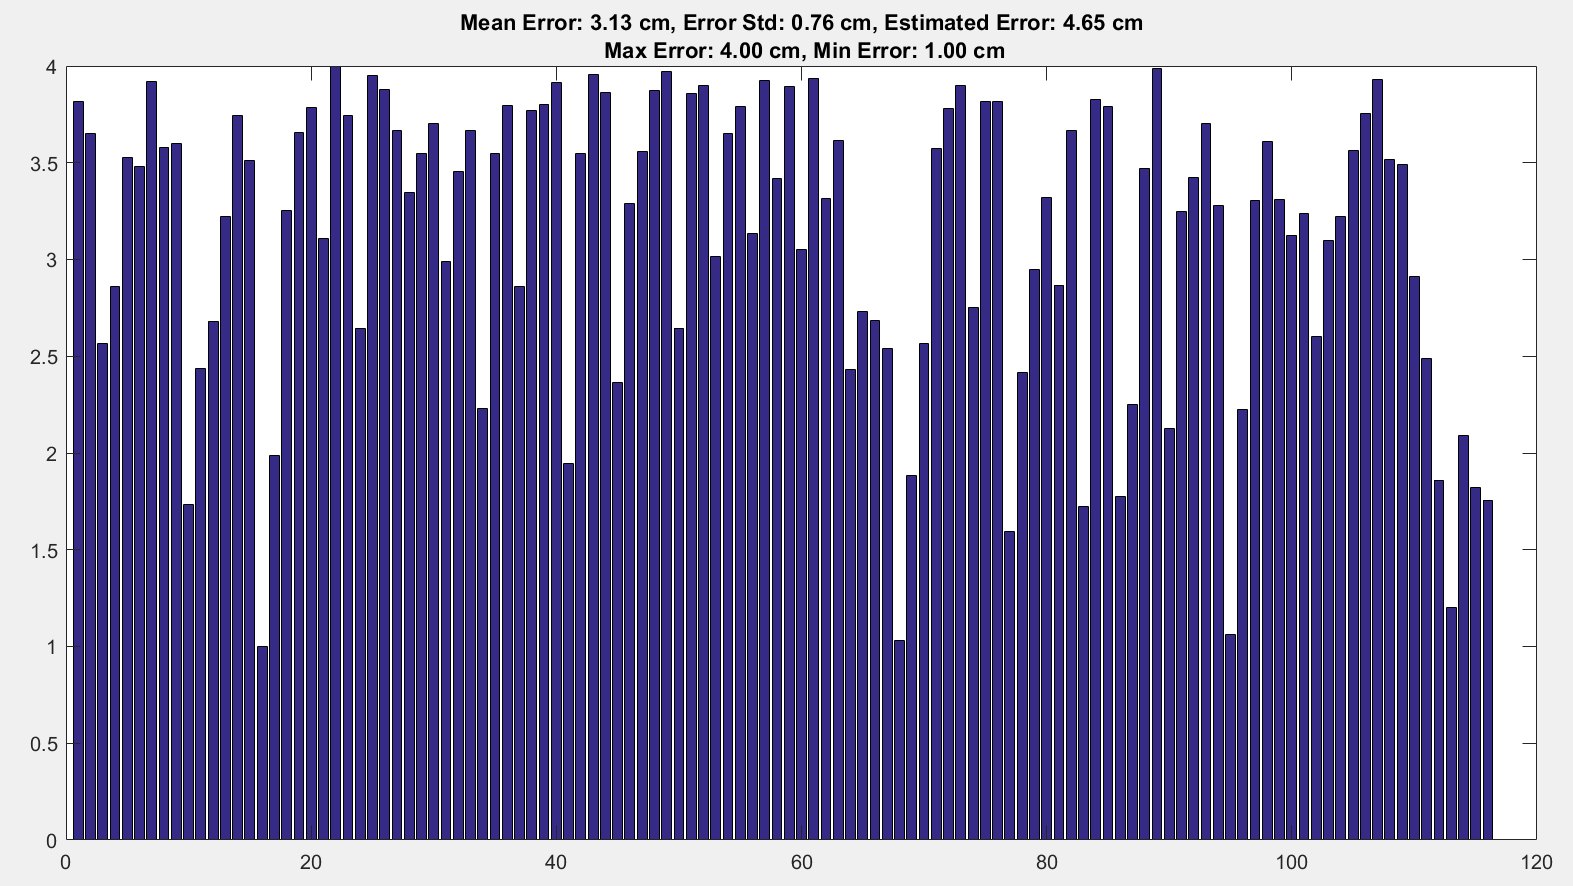
\includegraphics[scale=.25]{images/DATA-1599.PNG}
\caption{Results for robot motion with distanceThreshold = 15px and orientationThreshold = 0.99}
\label{fig:results3}
\end{figure}

As shown in these figures, the robot's path seems to follow the path drawn by the user.  Table~\ref{tab:error} shows these results in terms of standard deviation of error, mean error, maximum error, minimum error, and estimated error. Each of these values is converted to centimeters from pixels by using the known size of the workspace and the ArUco marker array.

\begin{table}[h!]
\caption{Error Analysis}
\label{tab:error}
\begin{tabular}{ | p{0.5cm} | p{0.5cm} | p{0.5cm} | p{0.75cm} | p{0.75cm} | p{0.75cm} | p{1cm} | }

\hline
	\textit{$a^*$} & \textit{$d^*$} & STD & Mean Error & Max Error & Min Error & Estimated Error \\ \hline
	0.95 & 20 & 0.68 & 4.82 & 5.56 & 1.30 & 6.19 \\ \hline
	0.99 & 20 & 0.68 & 4.76 & 5.55 & 2.83 & 6.11 \\ \hline
	0.99 & 15 & 0.76 & 3.13 & 4.01 & 1.00 & 4.65 \\ \hline
\hline    
\multicolumn{7}{ |c| }{Error in cm, $d^*$ in px} \\

\multicolumn{7}{ |c| }{\textit{$a^*$}= orientation threshold, \textit{$d^*$} = distance threshold} \\ \hline
\end{tabular}
\end{table}

As shown, as the threshold for orientation increased the estimated error decreased.  However, the largest contributor to the decrease in estimated error was the decrease in the distance threshold. Upon performing further tests, it was found that if the distance threshold is decreased then the orientation threshold must be increased, otherwise the robot would reach each point on the path but it will be unable to accurately produce the path due to the over-correction it will need to do. The orientation threshold contributes to lowering the over-correction needed. It was also found that lowering the distance threshold too much would result in the robot not being able to reach a point.  This is because while the ArUco marker detection is robust, it is not very stable and does shift by a few pixels causing errors in the system when the distance threshold is too small.  Another threshold needing to be modified was the time threshold.  This threshold was used to determine how often movement commands would be sent to the robot.  If it was too high the robot would overshoot points, if it was too low then the robot would get overloaded with commands. Therefore, a threshold of 50 ms was used after testing various values.


\chapter{Conclusions}
  ...
  \nocite{*}
%%%%%%%%%%%%%%%%%%%%%%%%%%%%%%%%%%%%%%%%%%%%%%%%%%%%%%%%%%%%%%%%%%%%%%%%%%%%%%%

%%%%%%%%%%%%%%%%%%%%%%%%%%%%%%%%%%%%%%%%%%%%%%%%%%%%%%%%%%%%%%%%%%%%%%%%%%%%%%%
\bibliographystyle{plain}
% Single space the bibliography to save space.
\begin{singlespace}
\bibliography{Thesis}
\end{singlespace}
%%%%%%%%%%%%%%%%%%%%%%%%%%%%%%%%%%%%%%%%%%%%%%%%%%%%%%%%%%%%%%%%%%%%%%%%%%%%%%%

%%%%%%%%%%%%%%%%%%%%%%%%%%%%%%%%%%%%%%%%%%%%%%%%%%%%%%%%%%%%%%%%%%%%%%%%%%%%%%%
% The appendices are (of course) optional.
\appendix
\chapter{A Long Proof}
  ...
%%%%%%%%%%%%%%%%%%%%%%%%%%%%%%%%%%%%%%%%%%%%%%%%%%%%%%%%%%%%%%%%%%%%%%%%%%%%%%%
\end{document}
